% ПРОЧИТАЙ МЕНЯ
% ПРОЧИТАЙ МЕНЯ
% ПРОЧИТАЙ МЕНЯ
%
% В этом файле вы описываете задачи из контеста
% Условия можно вставить в виде фотографий
% В идеях нужно написать хотя бы два-три предложения о задаче
% Если задача довольно трудная, описание идеи должно быть подробным
% Комментарии в исходном коде приветствуются
% Положение тоже можно фотографией
%
% ПРОЧИТАЙ МЕНЯ
% ПРОЧИТАЙ МЕНЯ
% ПРОЧИТАЙ МЕНЯ

\begin{center}
\bfseries{\large ТЕХНИЧЕСКИЙ ОТЧЁТ ПО ПРАКТИКЕ}
\end{center}

\subsection*{Основы C++ [1]}
\begin{center}
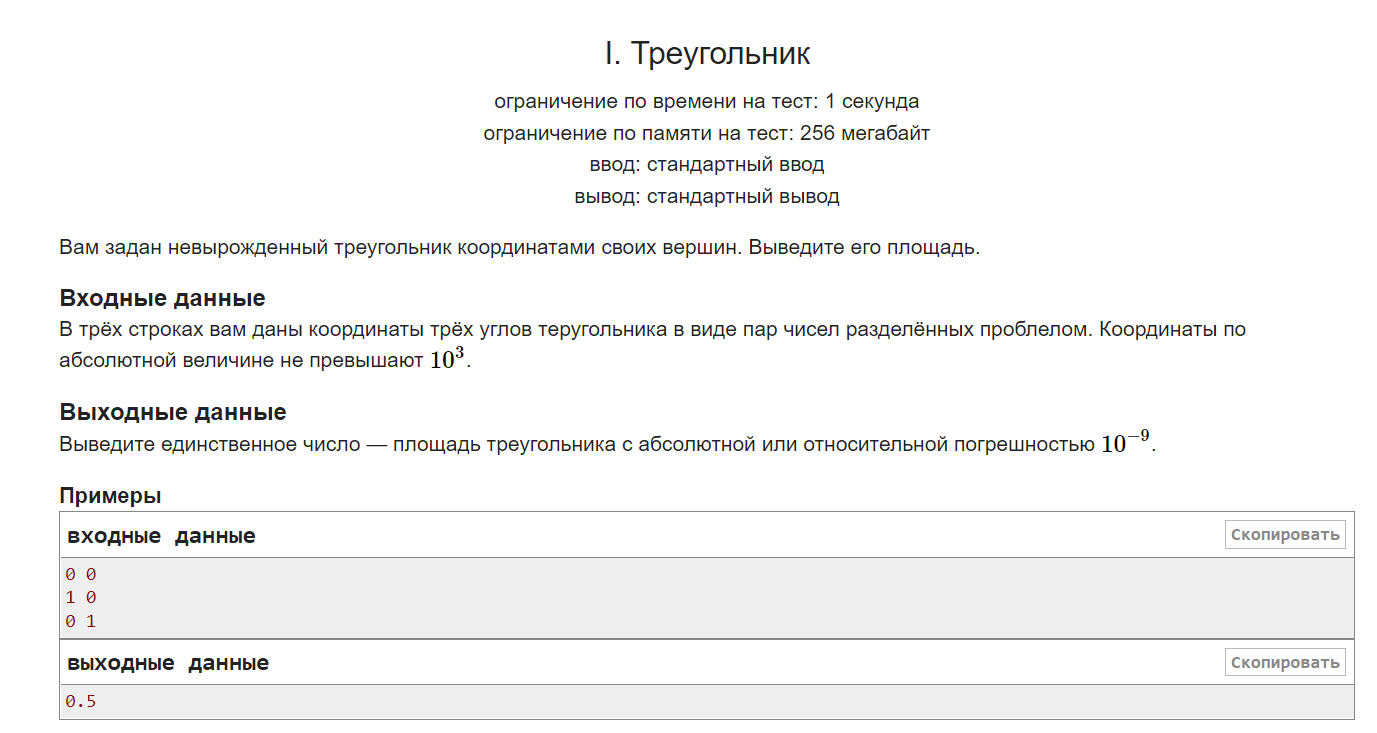
\includegraphics[width=\textwidth]{statements/1.png}
\end{center}
\subsubsection*{Идея решения}
Для того, чтобы определить площадь треугольника буду использовать формулу Герона:

$S=\sqrt{p(p-a)(p-b)(p-c)}$,

где $p$ - полупериметр треугольника, а $a$, $b$, $c$ - длины его сторон. Длину сторон вычислю по координатам вершин.

\subsubsection*{Исходный код}
\lstinputlisting{src/1.cpp}

\subsubsection*{Фрагмент турнирной таблицы контеста}
\begin{center}
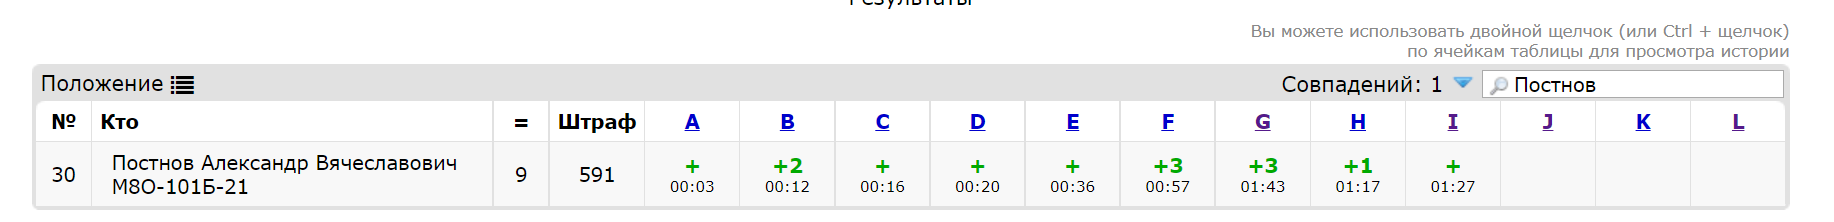
\includegraphics[width=\textwidth]{standings/1.png}\newline\noindent
\end{center}

\subsubsection*{Выводы}
Задача решена. Отладка не потребовалась.

\vspace{20pt}

\pagebreak
\subsection*{Основы C++ [2]}
\begin{center}
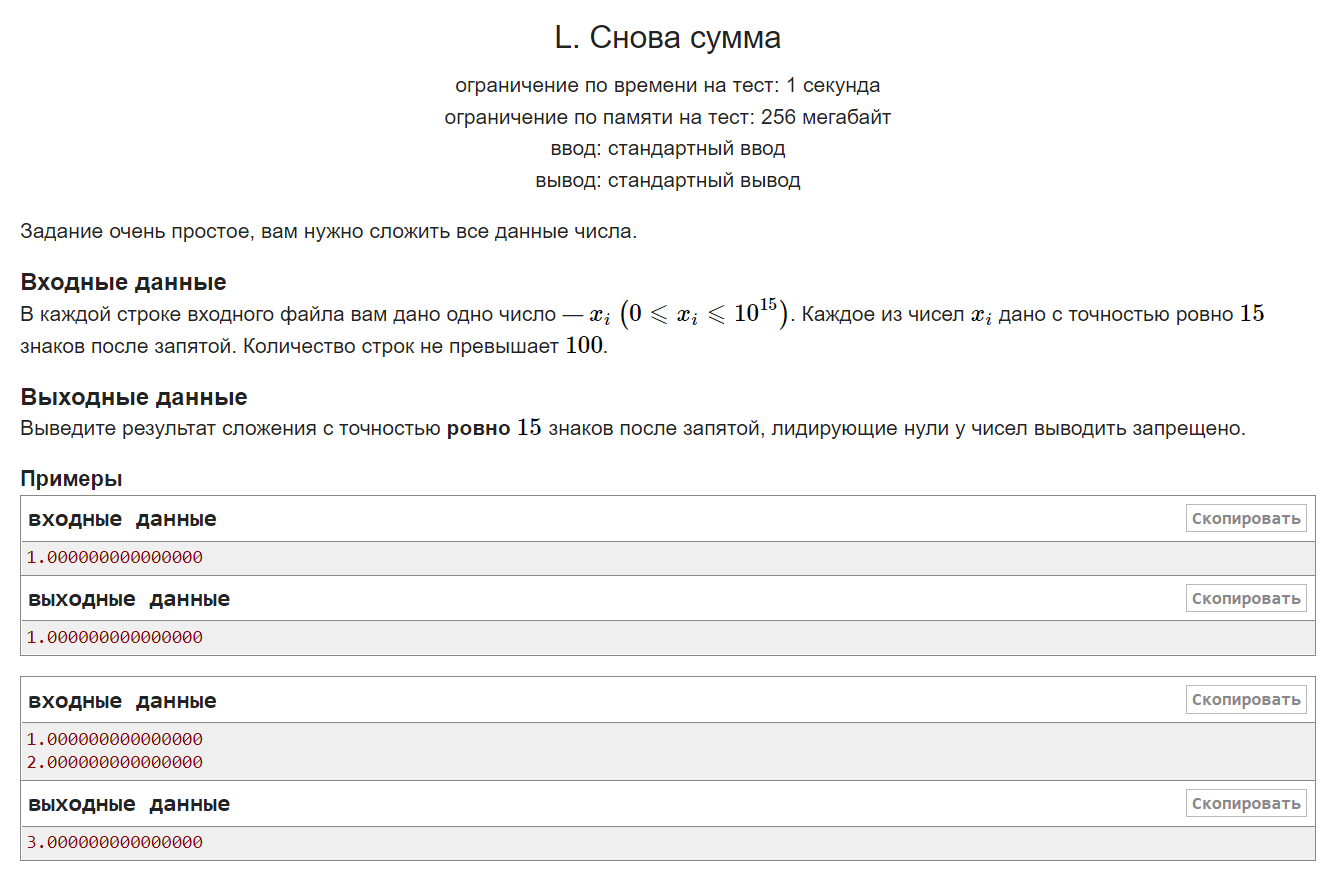
\includegraphics[width=\textwidth]{statements/2.png}
\end{center}
\subsubsection*{Идея решения}
В переменную типа $double$ не поместится такое длинное число, поэтому буду считать отдельно целую часть и вещественную часть. Ответом будет конкатенация этих строк.

\subsubsection*{Исходный код}
\lstinputlisting{src/2.cpp}

\subsubsection*{Фрагмент турнирной таблицы контеста}
\begin{center}
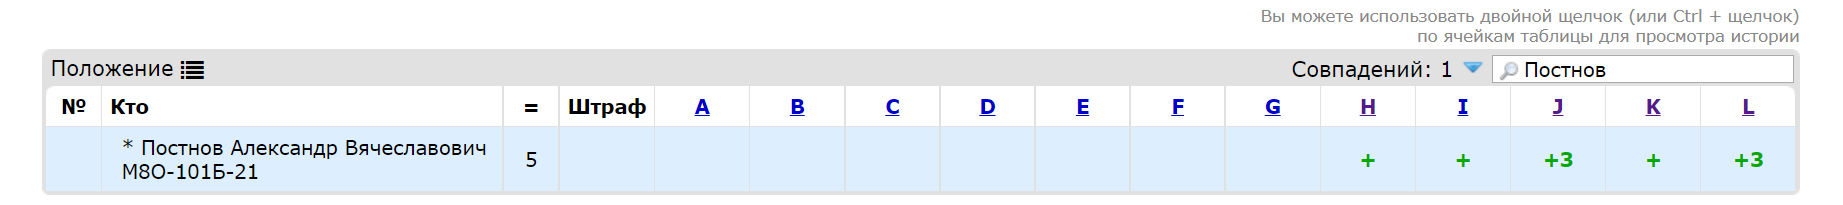
\includegraphics[width=\textwidth]{standings/2.png}\newline\noindent
\end{center}

\subsubsection*{Вывод}
Задача дорешана. Эта задача показывает, что нужно внимательно смотреть на входные данные.

\vspace{20pt}

\pagebreak

\subsection*{Библиотека C++ [3]}
\begin{center}
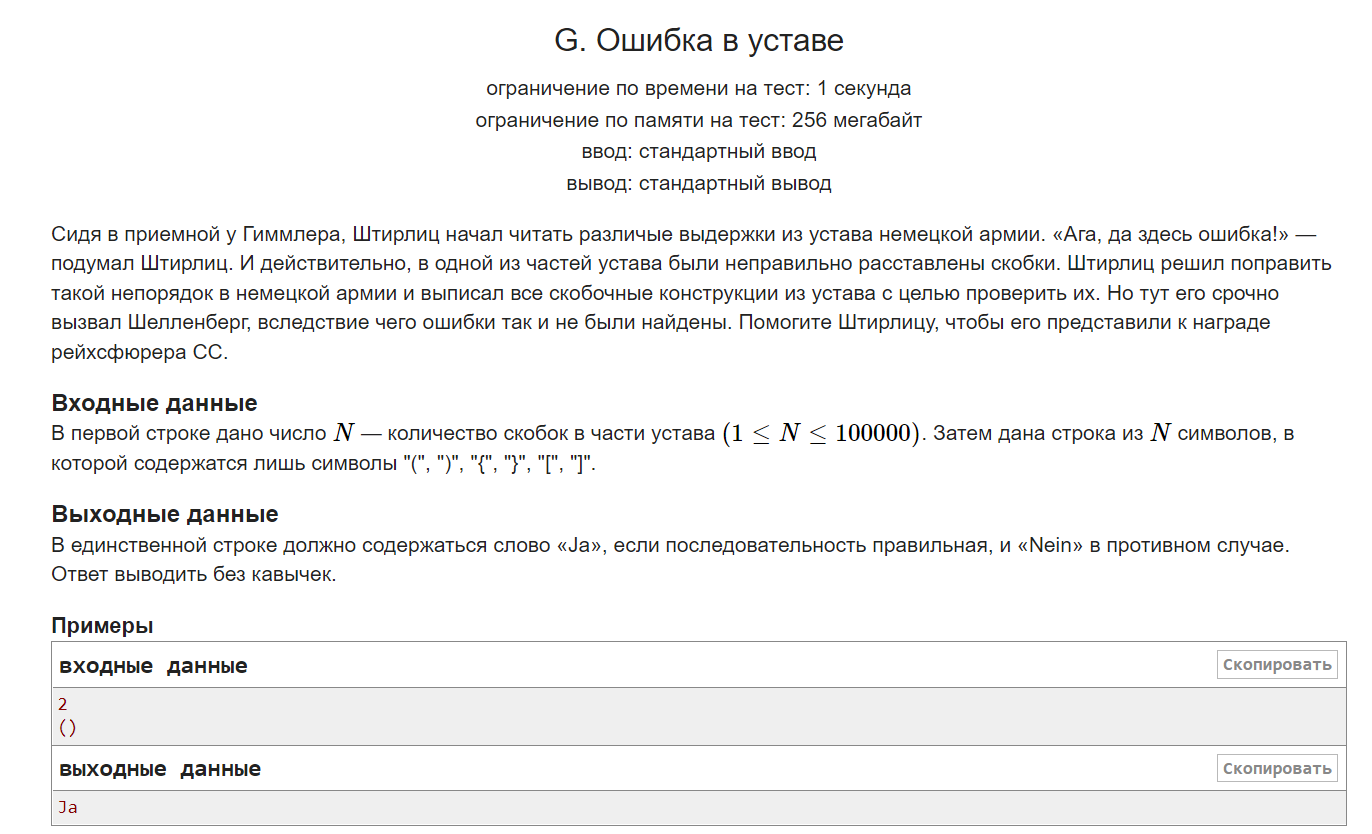
\includegraphics[width=\textwidth]{statements/3.png}
\end{center}
\subsubsection*{Идея решения}
Классическая задача на использование дека. Пушим открыв. скобки. Если на вход закрыв. скобка, попаем элемент из дека, проверяем на одинаковость типа открыв. скобки. $O(n)$

\subsubsection*{Исходный код}
\lstinputlisting{src/3.cpp}

\subsubsection*{Фрагмент турнирной таблицы контеста}
\begin{center}
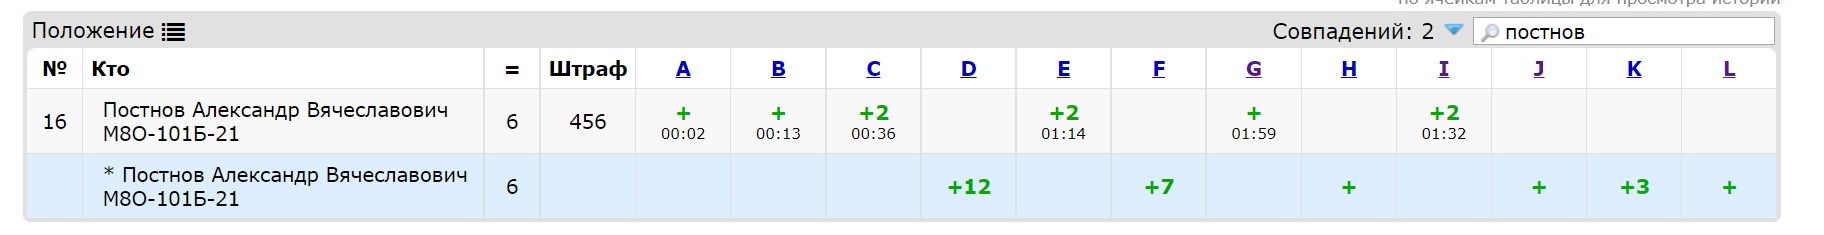
\includegraphics[width=\textwidth]{standings/3.png}\newline\noindent
\end{center}

\subsubsection*{Вывод}
Задача решена.

\vspace{20pt}

\pagebreak

\subsection*{Библиотека C++ [4]}
\begin{center}
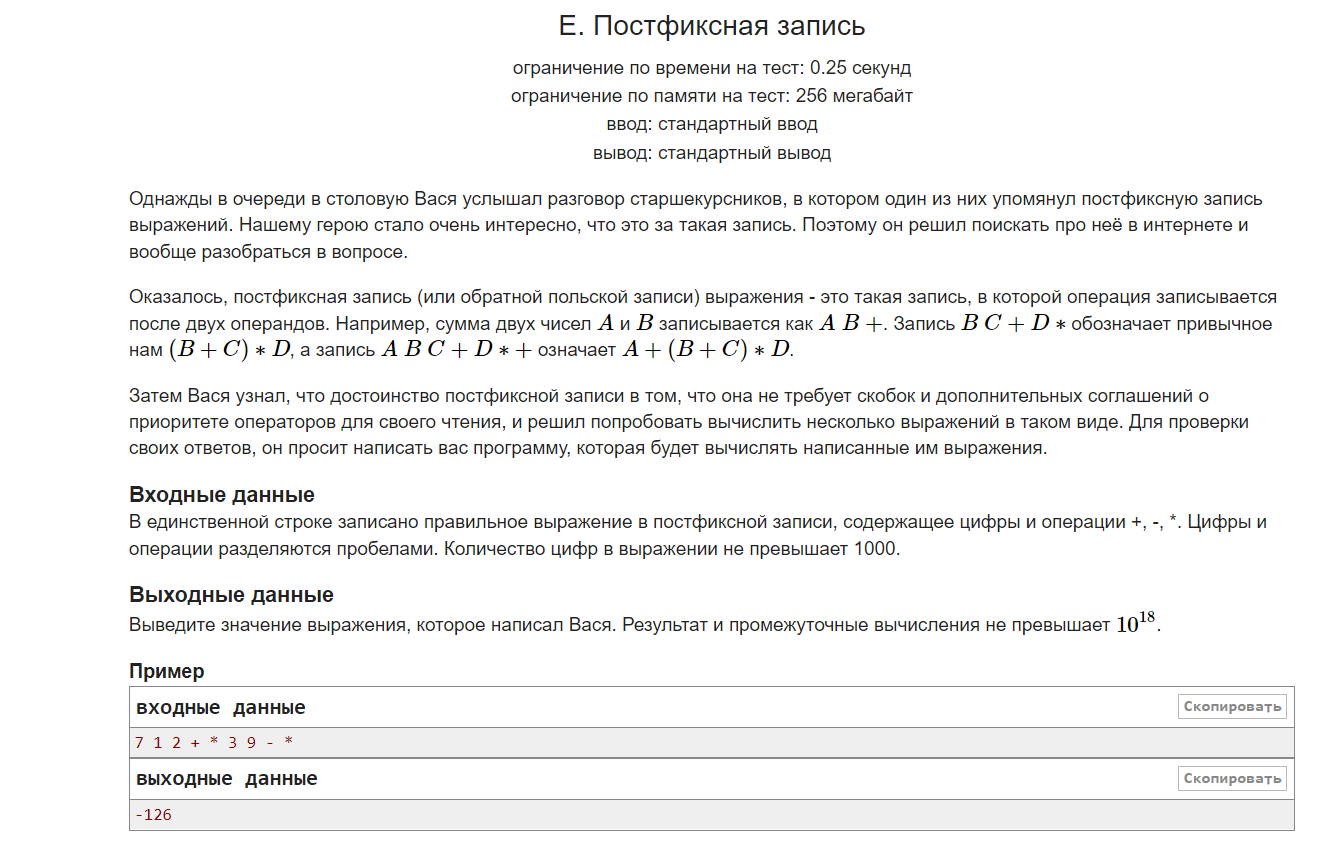
\includegraphics[width=\textwidth]{statements/4.png}
\end{center}
\subsubsection*{Идея решения}
Очередная задача на использование дека. Пушим числа в дек, если встречаем знак операции, то попаем 2 числа из дека и производим действие над числами, ответ пушим обратно в дек.
Итоговая сложность: $O(n)$

\subsubsection*{Исходный код}
\lstinputlisting{src/4.cpp}

\subsubsection*{Фрагмент турнирной таблицы контеста}
\begin{center}
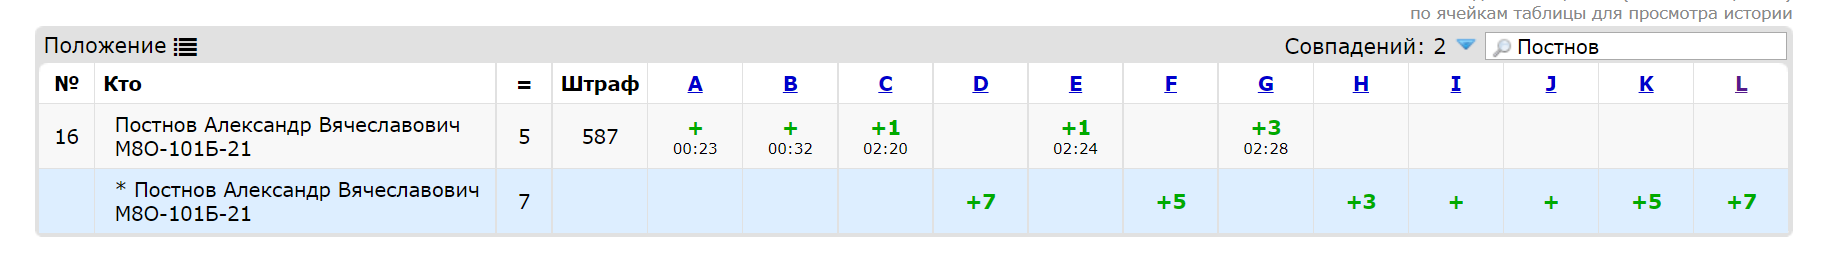
\includegraphics[width=\textwidth]{standings/4.png}\newline\noindent
\end{center}

\subsubsection*{Вывод}
Задача решена.

\vspace{20pt}

\pagebreak

\subsection*{Теория чисел [5]}
\begin{center}
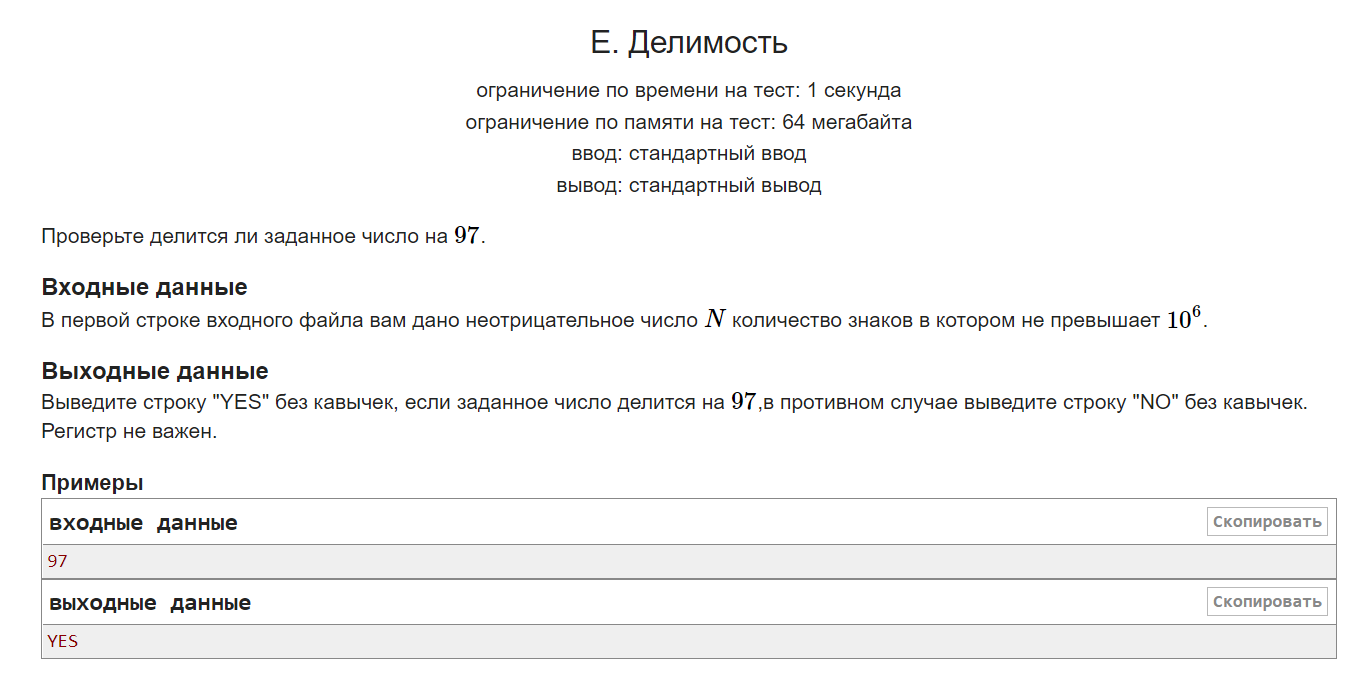
\includegraphics[width=\textwidth]{statements/5.png}
\end{center}
\subsubsection*{Идея решения}
Стоит обратить внимание, что кол-во знаков в числе $10^6$. Это означает, что число гигантское и нельзя взять просто остаток от деления. Значит, работаем с числом как со строкой, необходимо реализовать алгоритм деления в столбик. Итоговая сложность: $O(n)$, где $n$ - кол-во знаков в числе.

\subsubsection*{Исходный код}
\lstinputlisting{src/5.cpp}

\subsubsection*{Фрагмент турнирной таблицы контеста}
\begin{center}
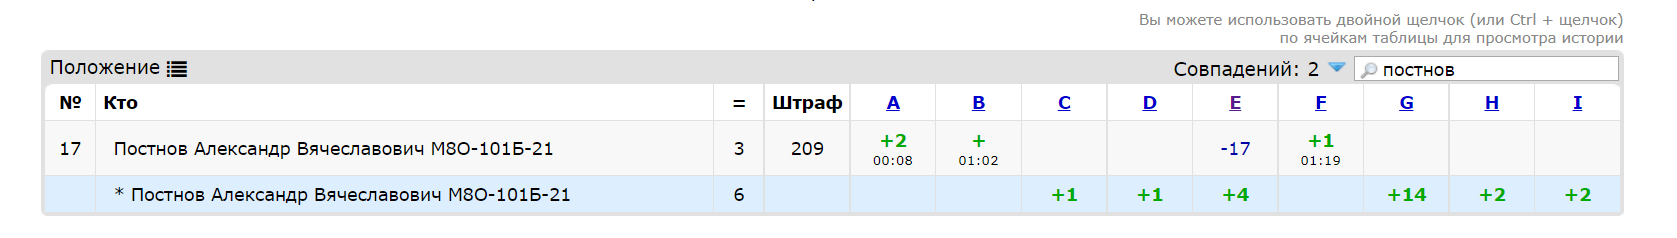
\includegraphics[width=\textwidth]{standings/5.png}\newline\noindent
\end{center}

\subsubsection*{Вывод}
Задача дорешена.

\vspace{20pt}

\pagebreak

\subsection*{Основы ДП [6]}
\begin{center}
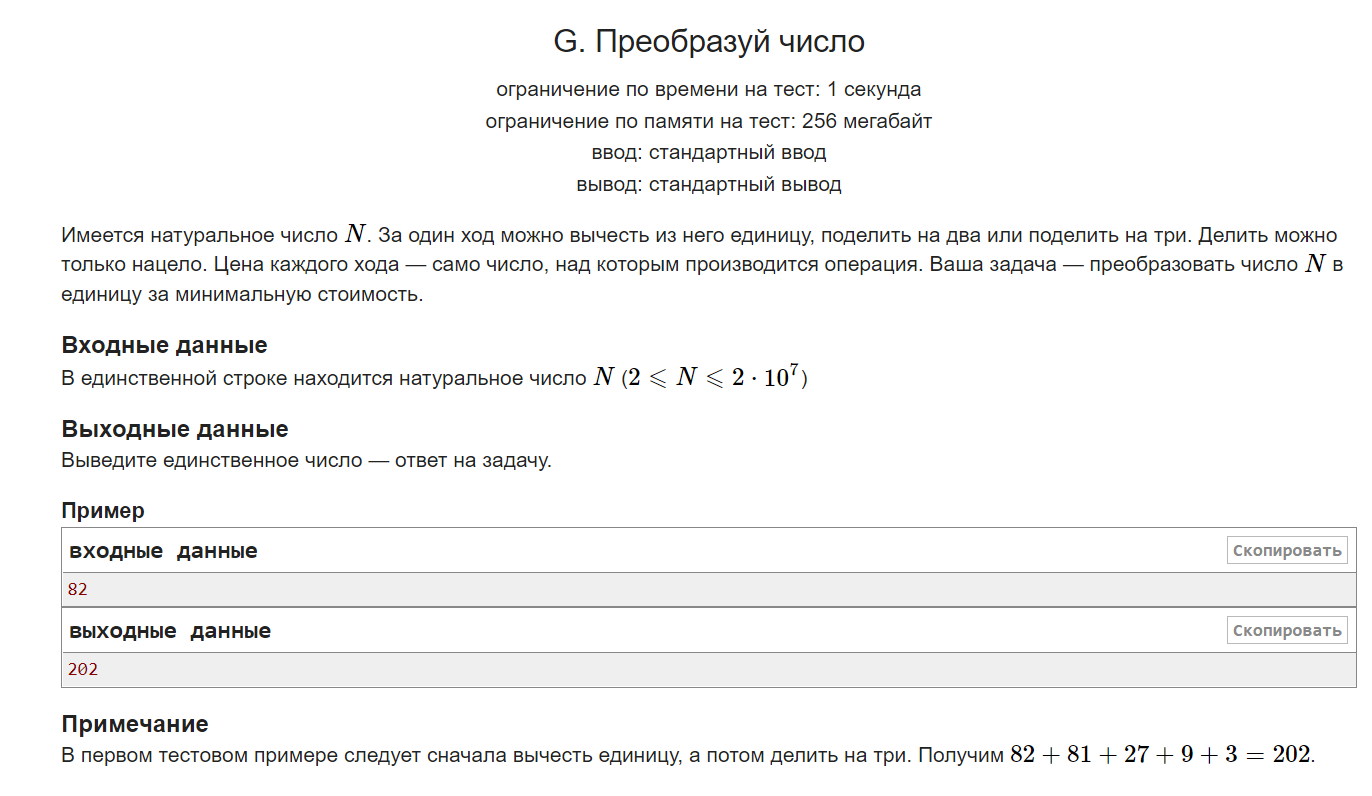
\includegraphics[width=\textwidth]{statements/6.png}
\end{center}
\subsubsection*{Идея решения}
В этой задаче стоит использовать идею динамического программирования. Создадим массив $a[n]$, в ячейках находится минимальная стоимость преобразования числа в 0, используя заданные операции. Просчитаем для всех чисел до n. Тогда разделим числа на 4 случая, когда число делится только на 2, только на 3, и на 2 и 3 одновременно и ни на что не делится. Рассмотрим случай например, когда число делится только на 2:
$a[i] = min(a[i / 2], a[i - 1]) + i$,
Аналогично для других случаев.
Ответ содержится в $a[n]$.
Итоговая сложность: $O(n)$
\subsubsection*{Исходный код}
\lstinputlisting{src/6.cpp}

\subsubsection*{Фрагмент турнирной таблицы контеста}
\begin{center}
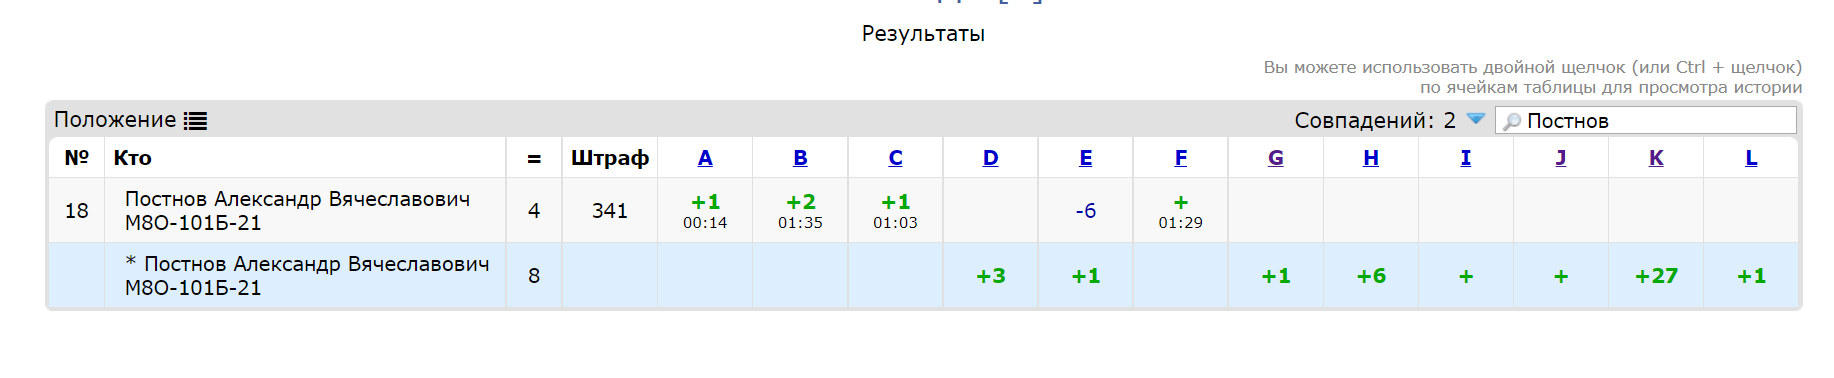
\includegraphics[width=\textwidth]{standings/6.png}\newline\noindent
\end{center}

\subsubsection*{Вывод}
Задача дорешена.

\vspace{20pt}

\pagebreak


\subsection*{Арифметика в кольце, комбинаторика, функция Эйлера [7]}
\begin{center}
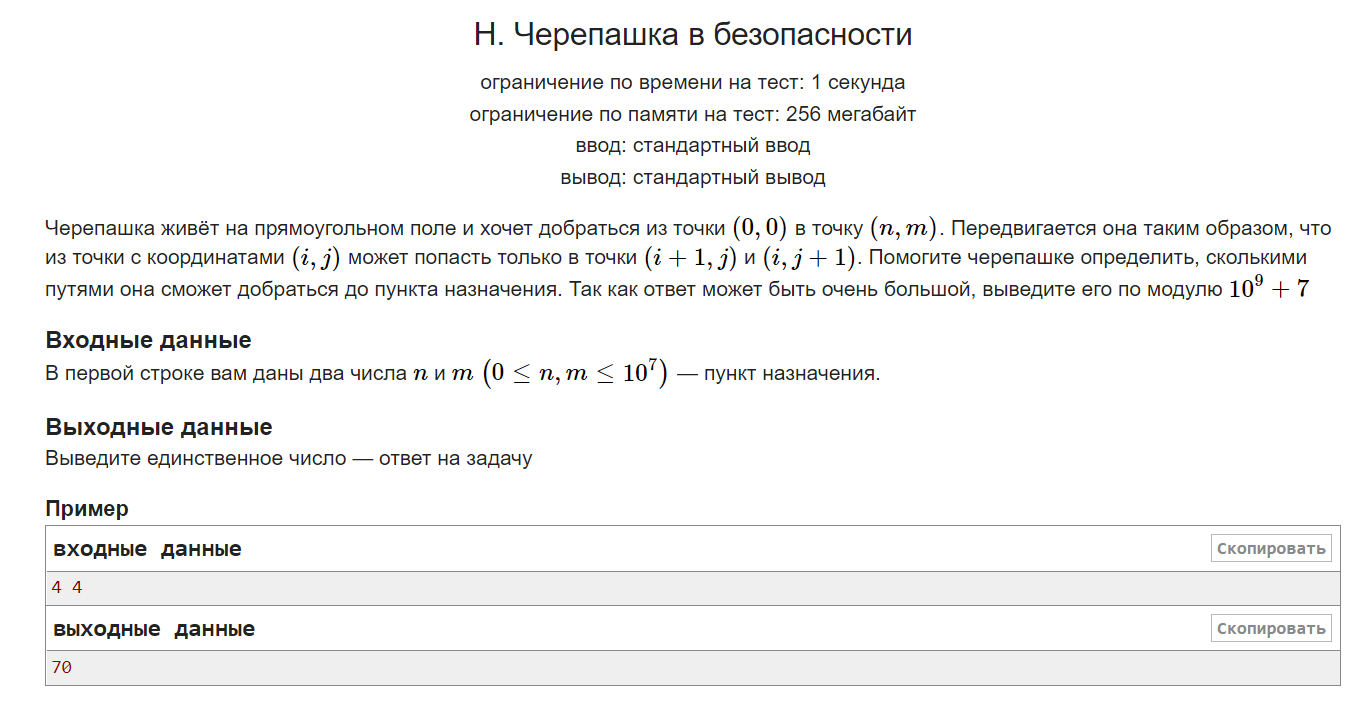
\includegraphics[width=\textwidth]{statements/7.png}
\end{center}
\subsubsection*{Идея решения}
Эту задачу можно решать с помощью динамического программирование, где в $a[i][j]$ хранится кол-во путей, чтобы в добраться в клетку с координатами $i, j$, но это слишком долго, так как итоговая сложность будет $O(n * m)$, а $n, m$ могут достигать $10^7$. Поэтому используем комбинаторику. Итоговый ответ - это $(n + m)!/(n!*m!)$
\subsubsection*{Исходный код}
\lstinputlisting{src/7.cpp}

\subsubsection*{Фрагмент турнирной таблицы контеста}
\begin{center}
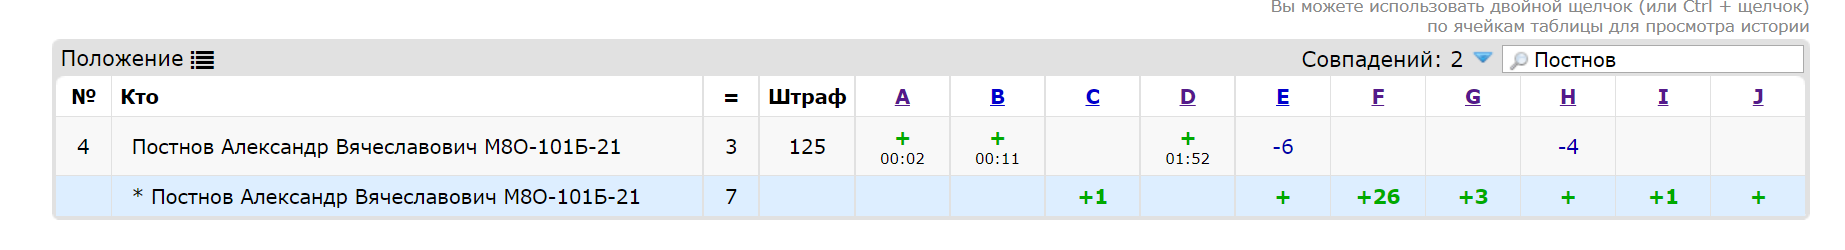
\includegraphics[width=\textwidth]{standings/7.png}\newline\noindent
\end{center}

\subsubsection*{Вывод}
Задача дорешена.

\vspace{20pt}

\pagebreak

\subsection*{Префиксные суммы, сортировка событий, метод двух указателей [8]}
\begin{center}
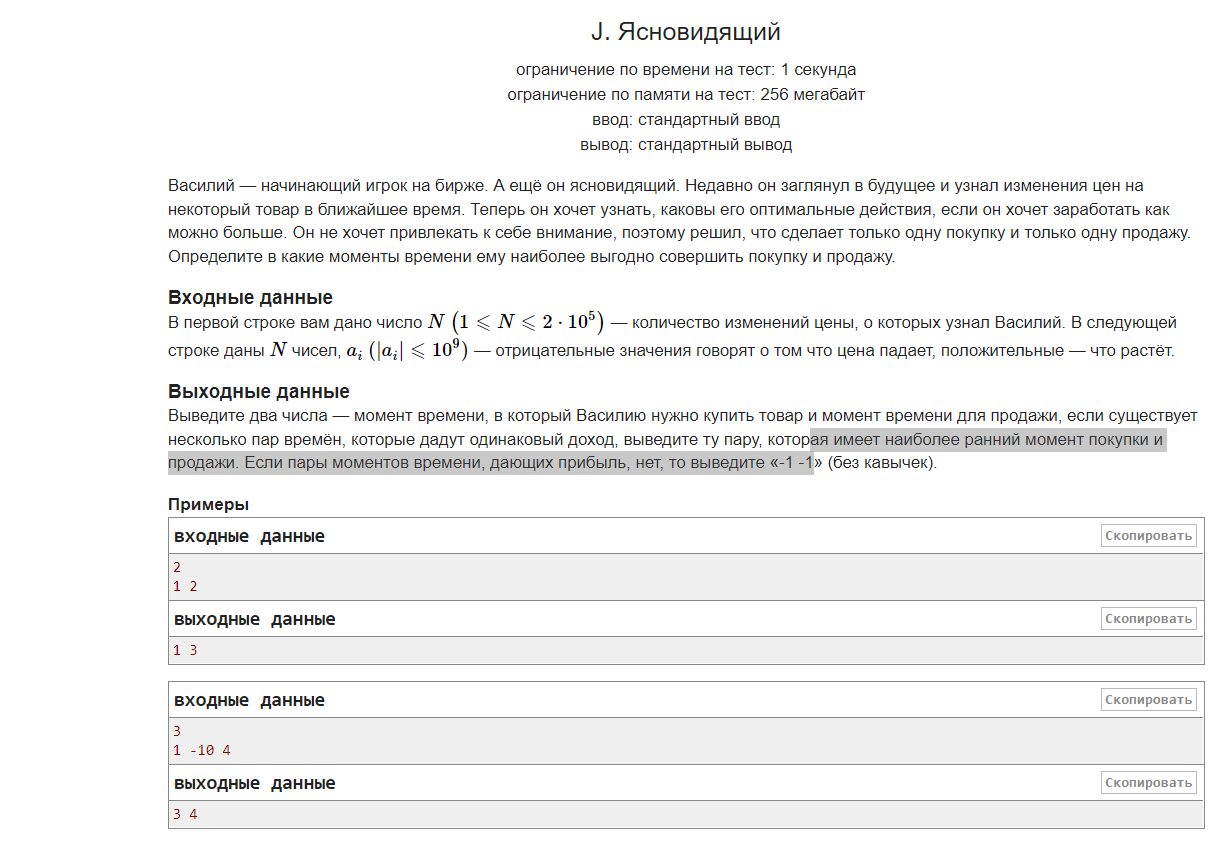
\includegraphics[width=\textwidth]{statements/8.png}
\end{center}
\subsubsection*{Идея решения}
Буду использовать метод двух указателей. Первый указатель следит за минимумом, а второй проходит по массиву. Если разница между текущим числом и миним. максимальная, запоминаем позиции минимума и текущего числа. Итоговая сложность: $O(n)$
\subsubsection*{Исходный код}
\lstinputlisting{src/8.cpp}

\subsubsection*{Фрагмент турнирной таблицы контеста}
\begin{center}
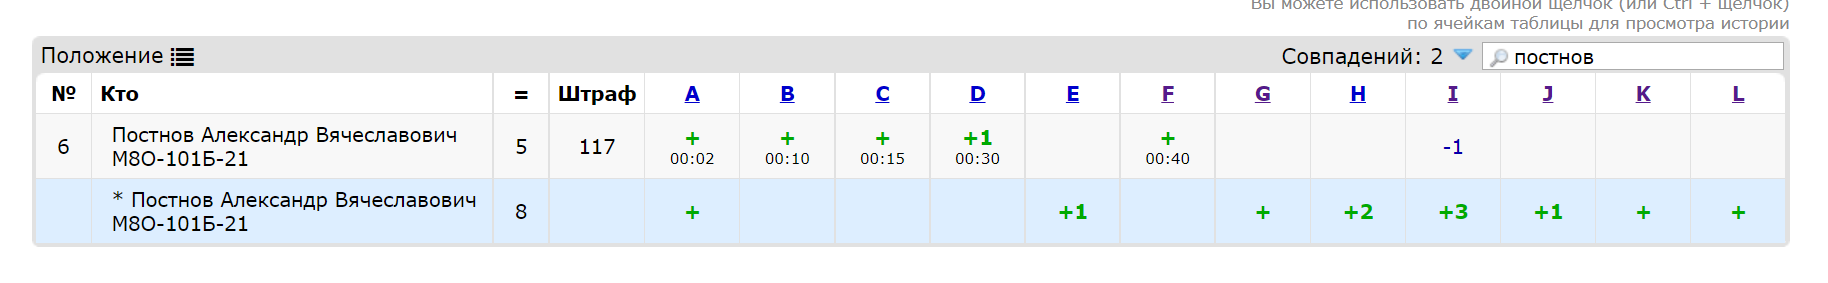
\includegraphics[width=\textwidth]{standings/8.png}\newline\noindent
\end{center}

\subsubsection*{Вывод}
Задача дорешена.

\vspace{20pt}

\pagebreak

\subsection*{Двумерное ДП, задача о рюкзаке [9]}
\begin{center}
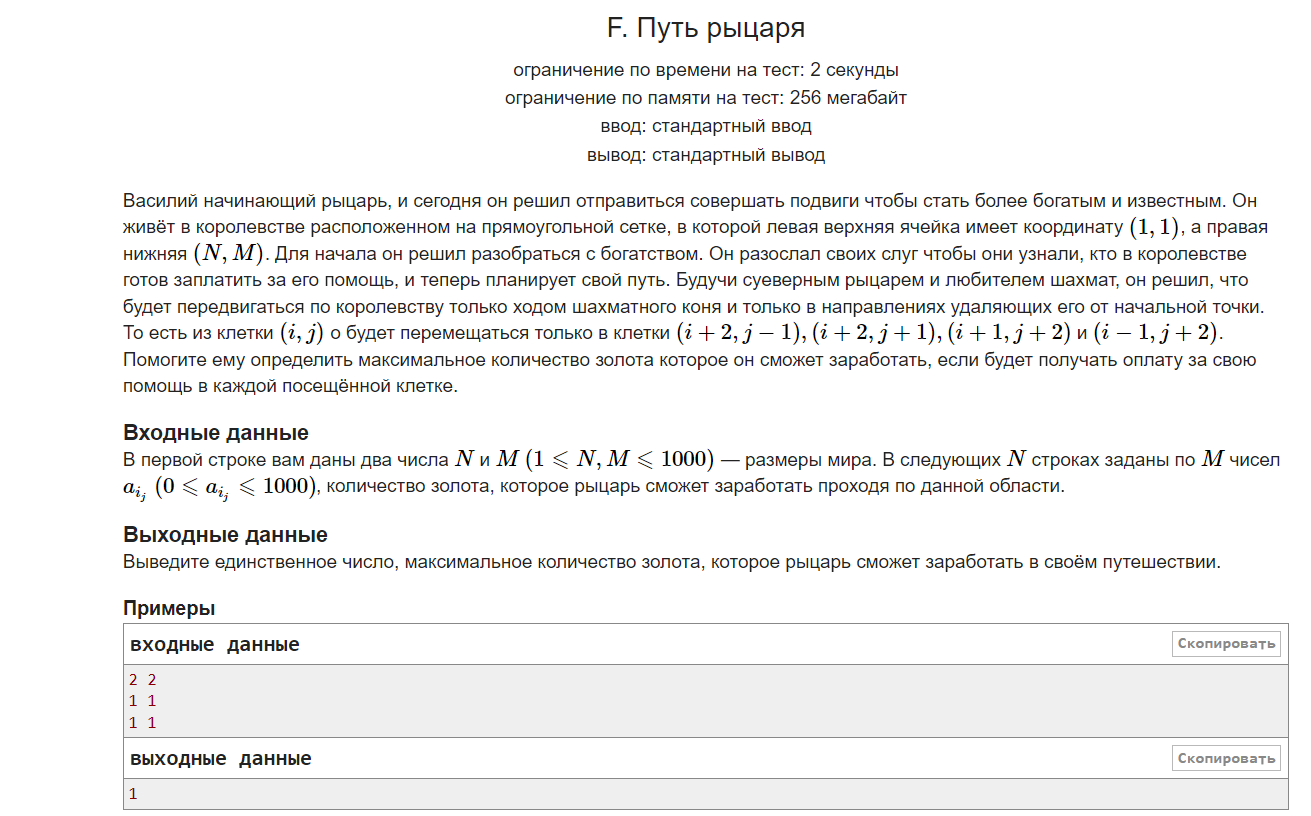
\includegraphics[width=\textwidth]{statements/9.png}
\end{center}
\subsubsection*{Идея решения}
В этой задаче нужно использовать метод ДП, в ячейке $a[i][j]$ будет храниться максимальное кол-во золота, которое он может заработать. Так как путь рыцаря довольно сложно реализуемый на циклах, буду использовать рекурсию, чтобы она была эффективной, буду проверять, что клетка не была посещена. Итоговая сложность: $O(n * m)$
\subsubsection*{Исходный код}
\lstinputlisting{src/9.cpp}

\subsubsection*{Фрагмент турнирной таблицы контеста}
\begin{center}
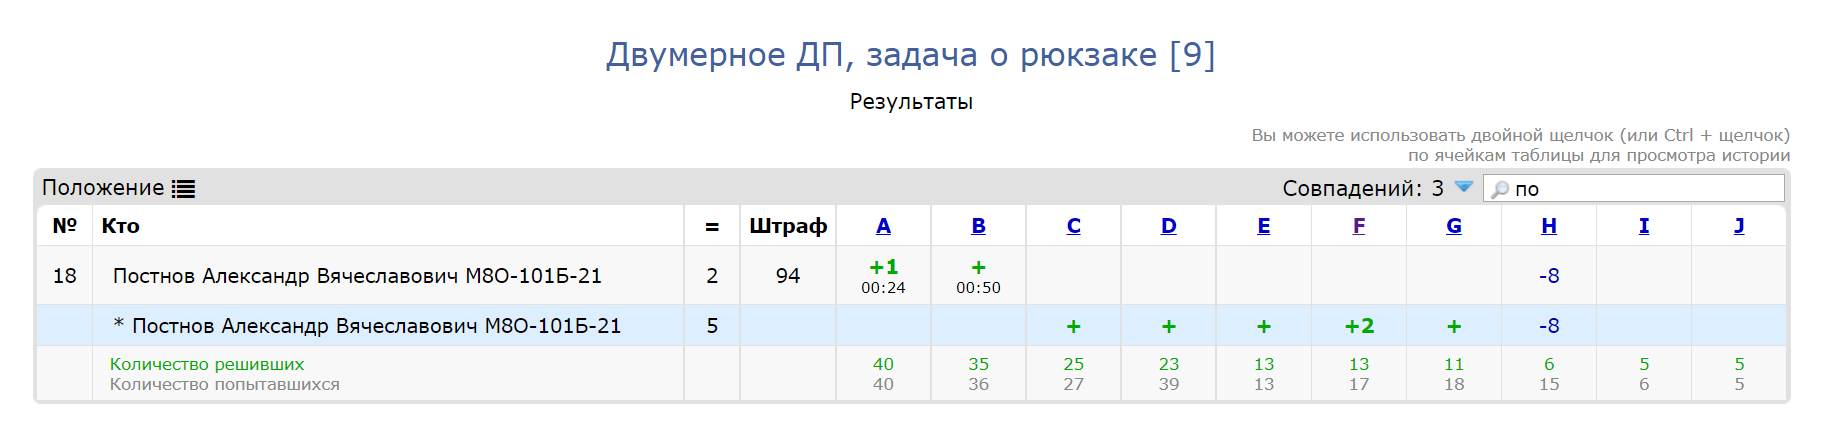
\includegraphics[width=\textwidth]{standings/9.png}\newline\noindent
\end{center}

\subsubsection*{Вывод}
Задача дорешена.

\vspace{20pt}

\pagebreak

\subsection*{Геометрия, тернарный поиск [10]}
\begin{center}
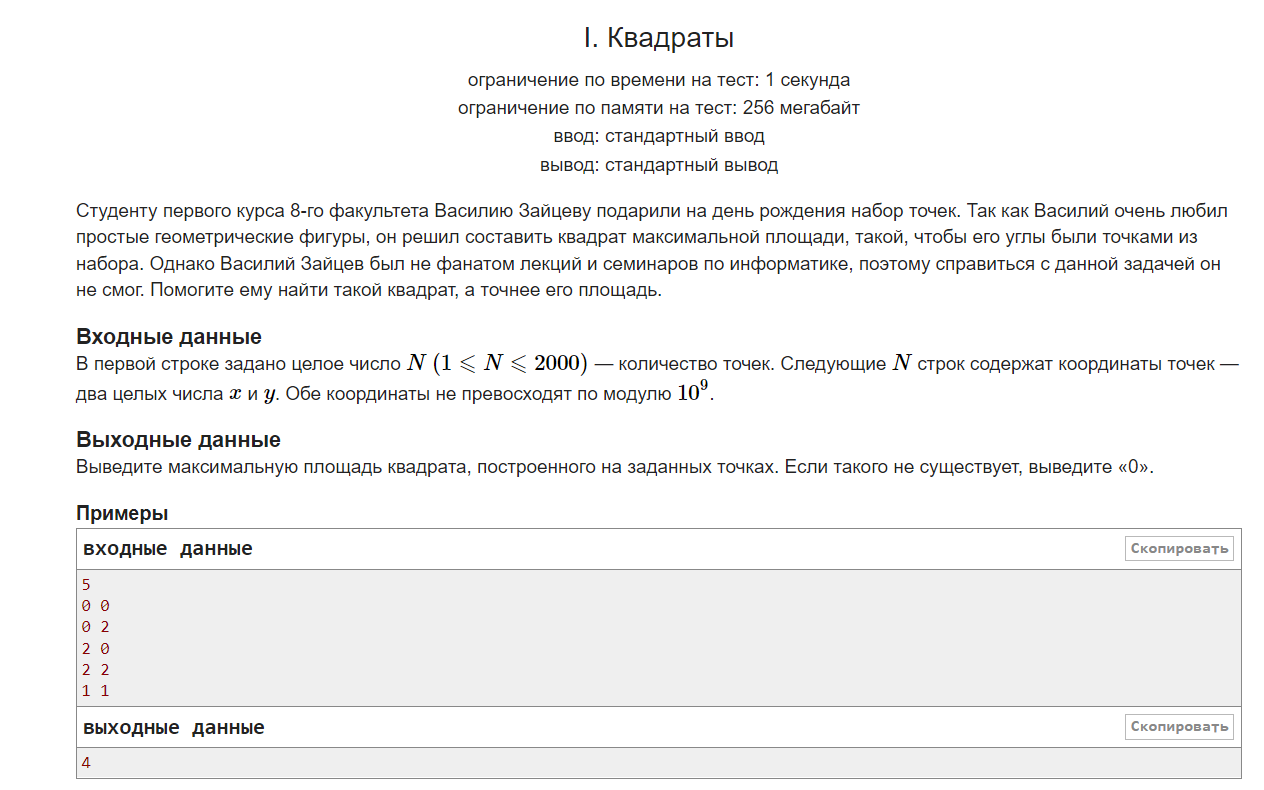
\includegraphics[width=\textwidth]{statements/10.png}
\end{center}
\subsubsection*{Идея решения}
Зафиксирую 2 координаты и построю по ним квадрат. 2 другие координаты могут быть расположены 2 способами. Вычисляю площадь. Если один из способов присутствует в множестве координат, значит построить квадрат именно так возможно. Обновляю по необходимости ответ. Итоговая сложность: $O(n^2*\log_{2} n)$
\subsubsection*{Исходный код}
\lstinputlisting{src/10.cpp}

\subsubsection*{Фрагмент турнирной таблицы контеста}
\begin{center}
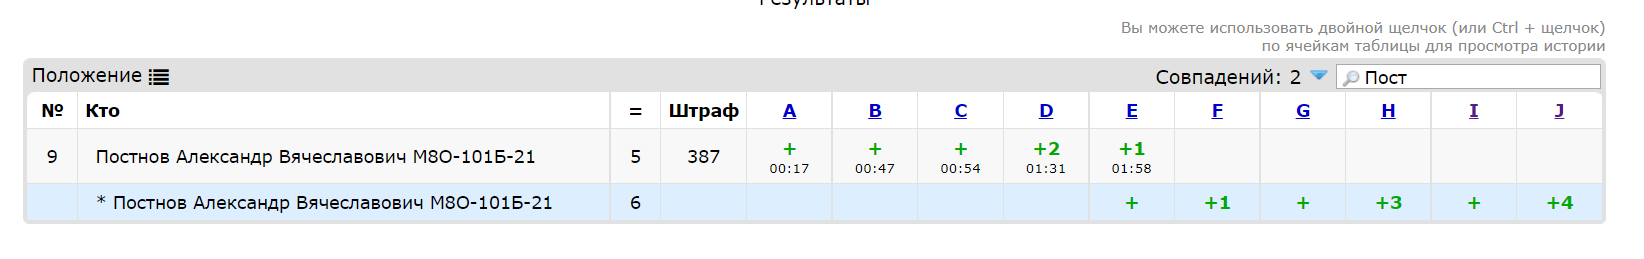
\includegraphics[width=\textwidth]{standings/10.png}\newline\noindent
\end{center}

\subsubsection*{Вывод}
Задача дорешена.

\vspace{20pt}

\pagebreak

\subsection*{Осенняя олимпиада первого курса}
\begin{center}
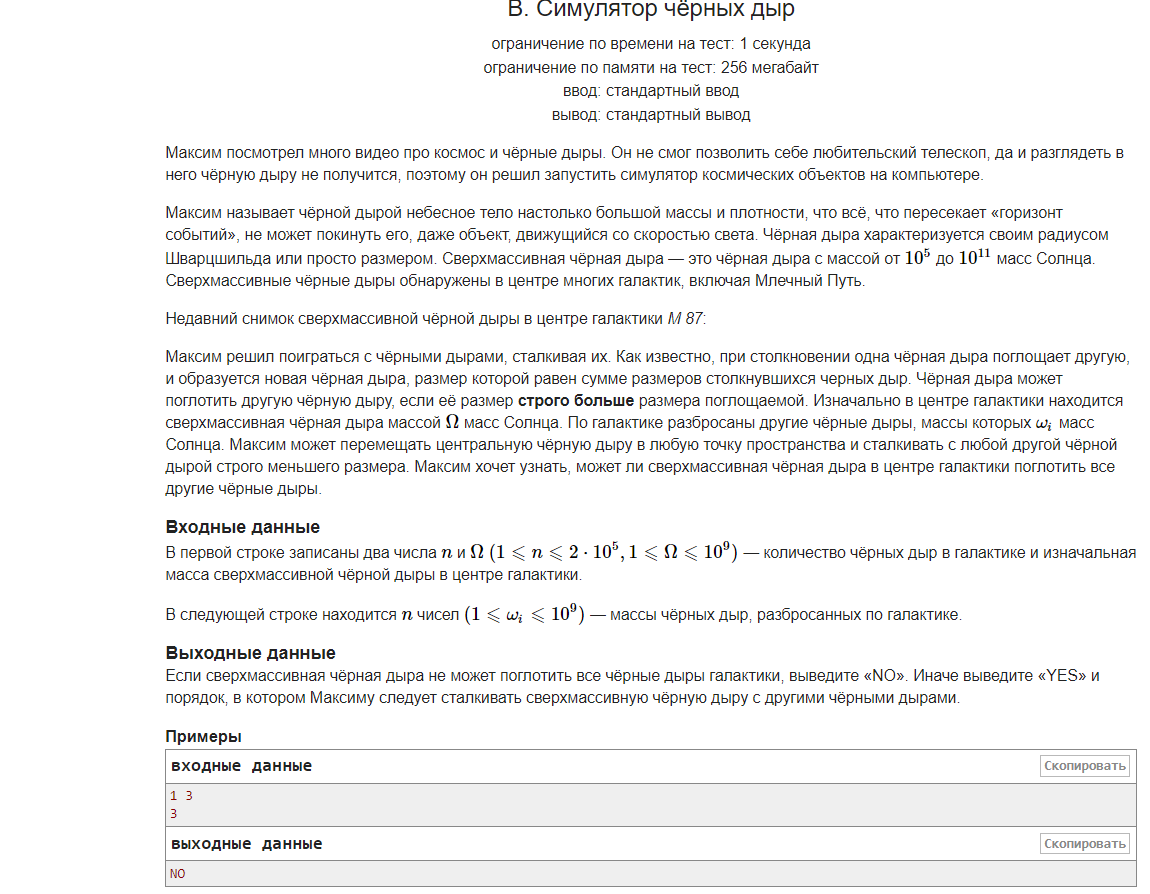
\includegraphics[width=\textwidth]{statements/11.png}
\end{center}
\subsubsection*{Идея решения}
Чтобы знать в каком порядке черная дыра поглощала другие дыры, необходимо создать структуру, в которой содержится ее масса и номер. Сортируем дыры по массе. И идем от меньшей к большей. Проверяем, может ли наша дыра съесть текущую дыру, если нет, то ответ на задачу нет, если да, то поглощаем и продвигаемся дальше. Итоговая сложность: $O(n*\log_{2} n)$ (сложность сортировки)
\subsubsection*{Исходный код}
\lstinputlisting{src/11.cpp}

\subsubsection*{Фрагмент турнирной таблицы контеста}
\begin{center}
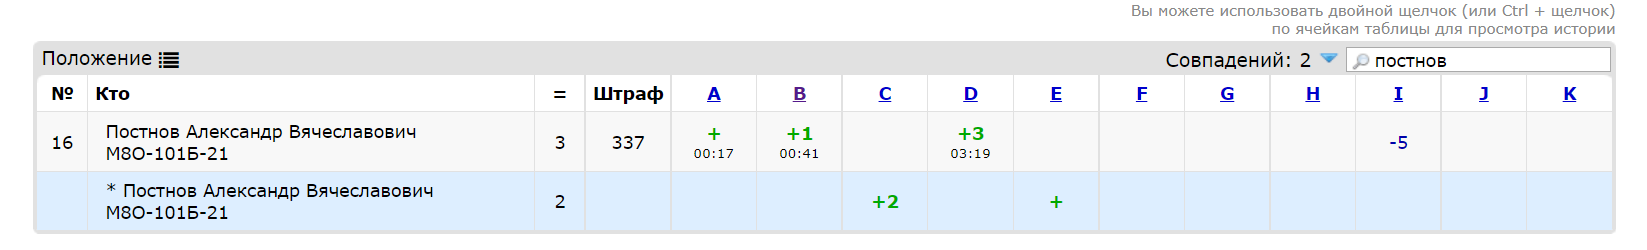
\includegraphics[width=\textwidth]{standings/11.png}\newline\noindent
\end{center}

\subsubsection*{Вывод}
Задача решена.

\vspace{20pt}

\pagebreak

\subsection*{Тренировочный контест на разные темы}
\begin{center}
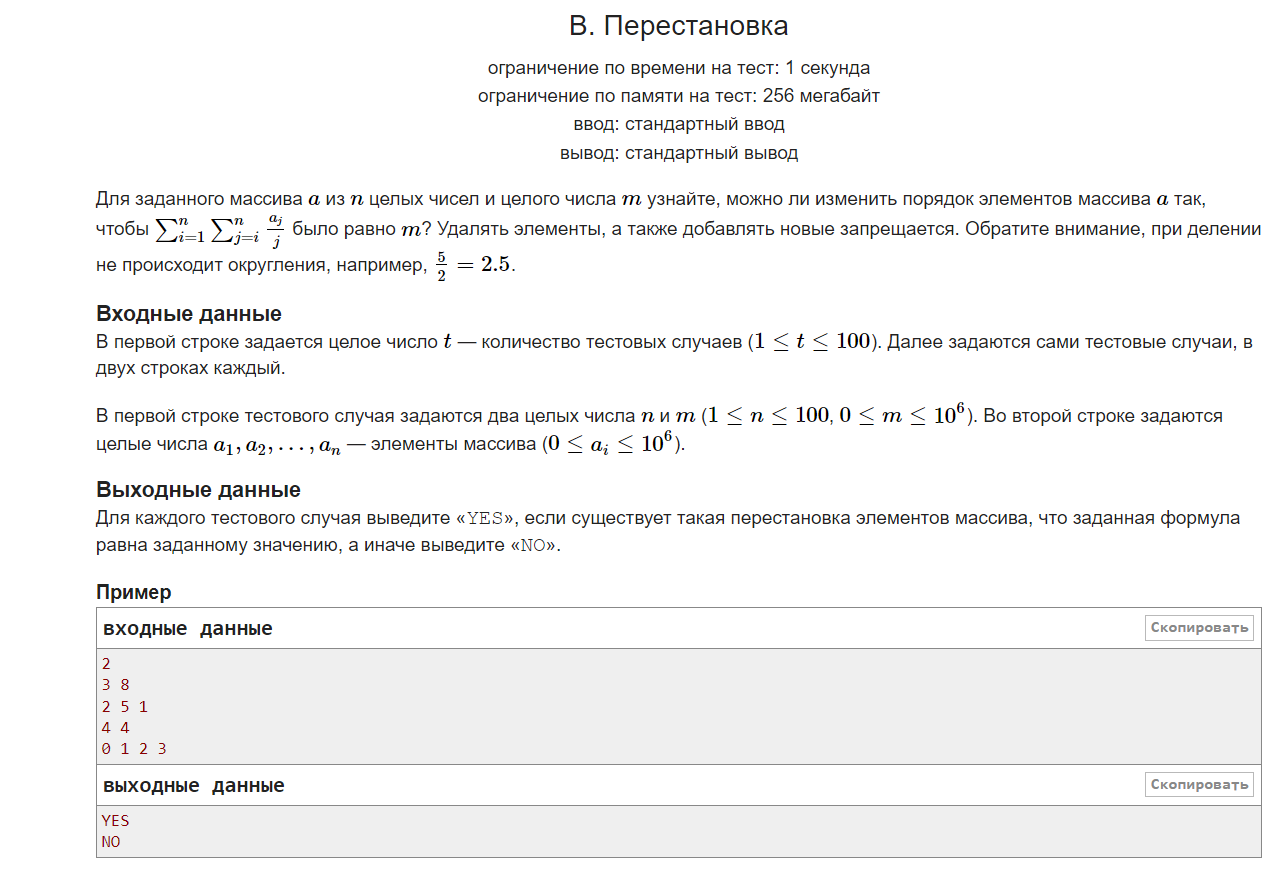
\includegraphics[width=\textwidth]{statements/12.png}
\end{center}
\subsubsection*{Идея решения}
Методом пристального взгляда можно определить, что формула в условии обозначает просто сумму элементов массива. Задача становится тривиальной. Итоговая сложность: $O(t*n)$
\subsubsection*{Исходный код}
\lstinputlisting{src/12.cpp}

\subsubsection*{Фрагмент турнирной таблицы контеста}
\begin{center}
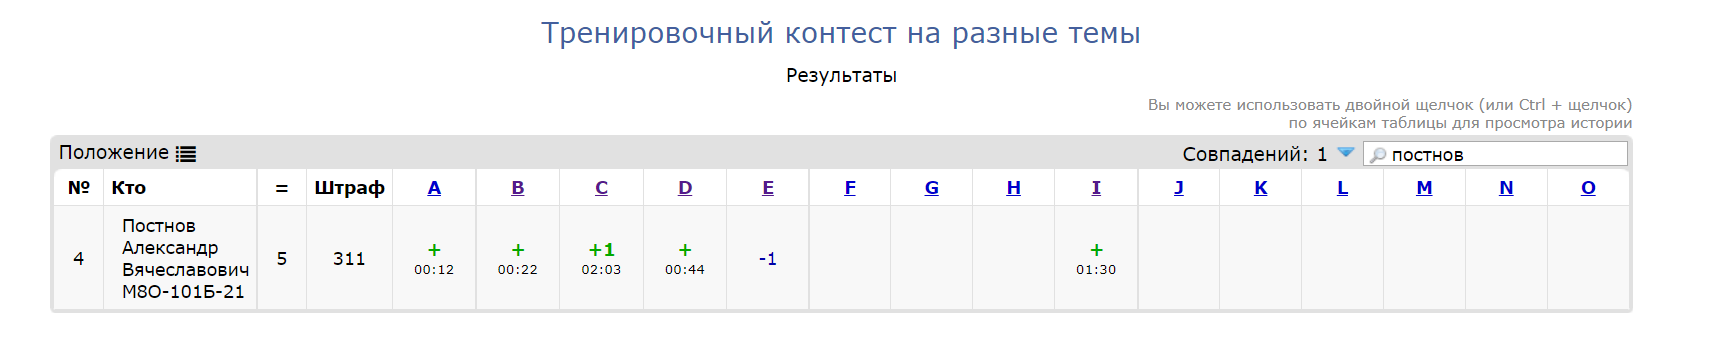
\includegraphics[width=\textwidth]{standings/12.png}\newline\noindent
\end{center}

\subsubsection*{Вывод}
Задача решена.

\vspace{20pt}

\pagebreak

\subsection*{Основы теории графов [11]}
\begin{center}
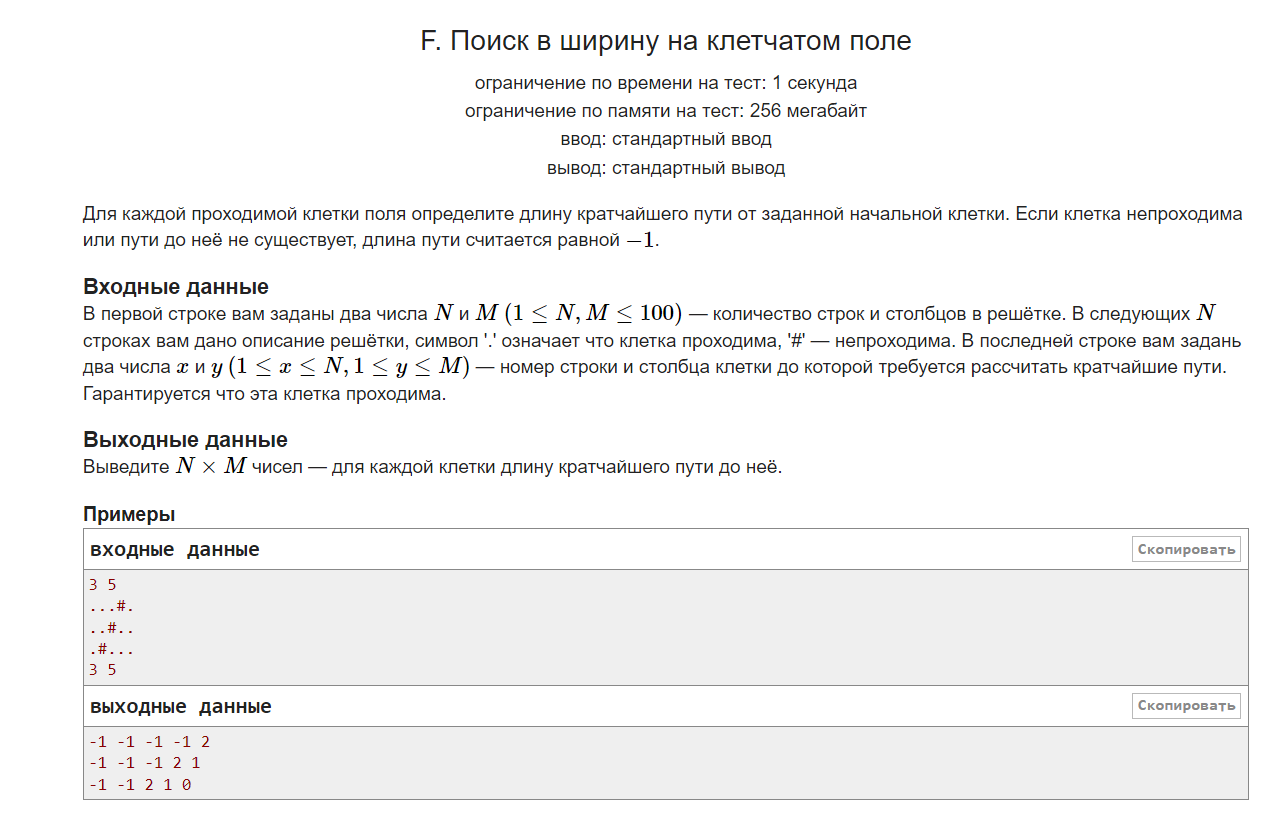
\includegraphics[width=\textwidth]{statements/13.png}
\end{center}
\subsubsection*{Идея решения}
Необходимо реализовать bfs для двумерного массива.
\subsubsection*{Исходный код}
\lstinputlisting{src/13.cpp}

\subsubsection*{Фрагмент турнирной таблицы контеста}
\begin{center}
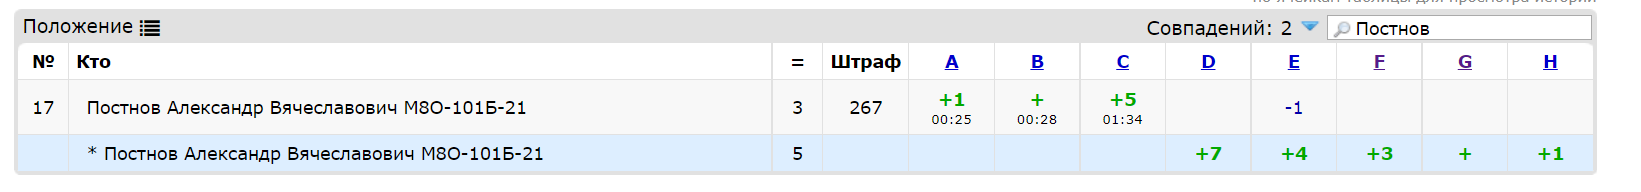
\includegraphics[width=\textwidth]{standings/13.png}\newline\noindent
\end{center}

\subsubsection*{Вывод}
Задача дорешена.

\vspace{20pt}

\pagebreak

\subsection*{Кратчайшие пути во взвешенных графах [12]}
\begin{center}
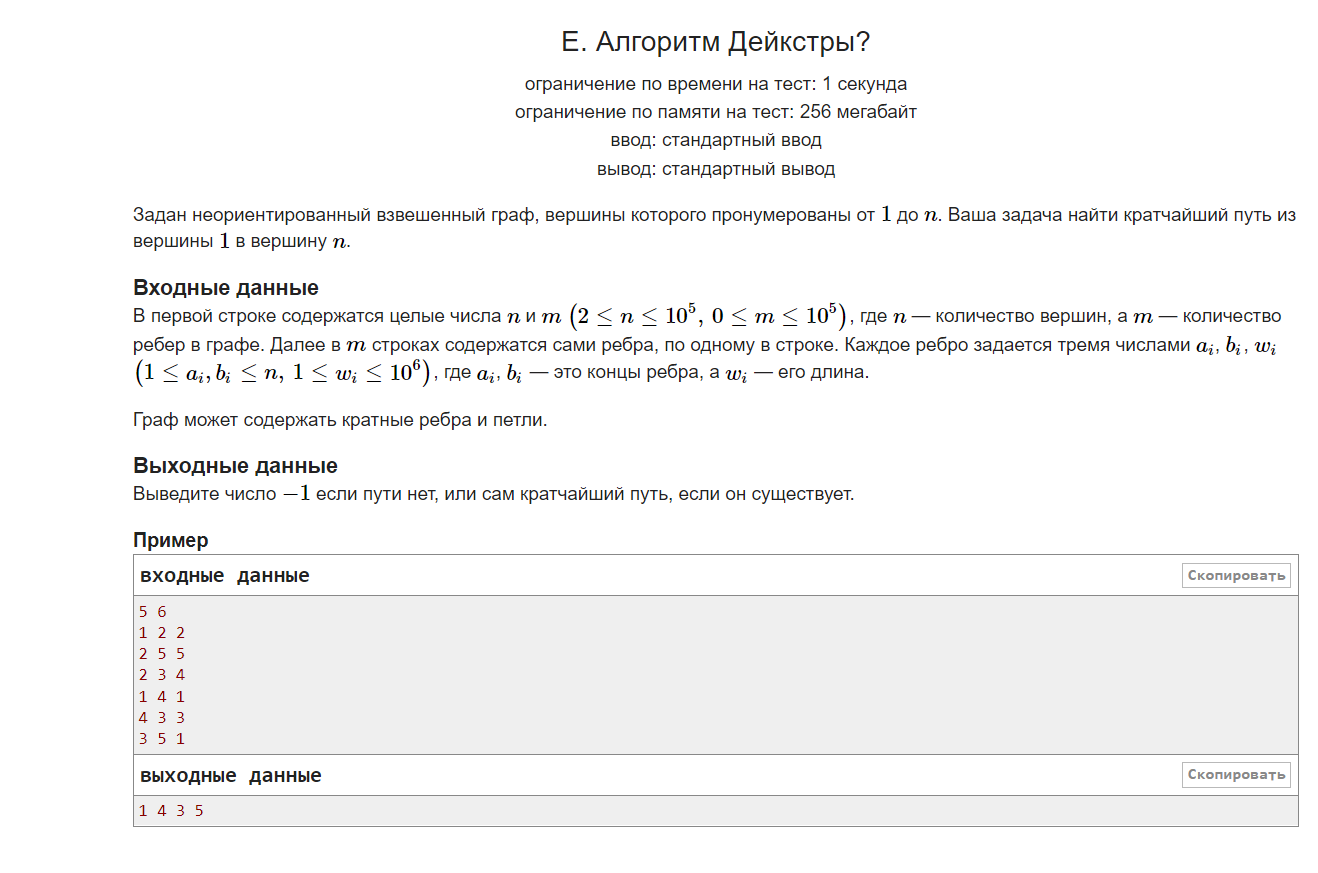
\includegraphics[width=\textwidth]{statements/14.png}
\end{center}
\subsubsection*{Идея решения}
Так как $n, m <= 10^5$ необходимо использовать алгоритм Дейкстры для разреженных графов. Чтобы вывести найденный путь, буду использовать массив предков.
Итоговая сложность: $O(m*\log_{2} n)$
\subsubsection*{Исходный код}
\lstinputlisting{src/14.cpp}

\subsubsection*{Фрагмент турнирной таблицы контеста}
\begin{center}
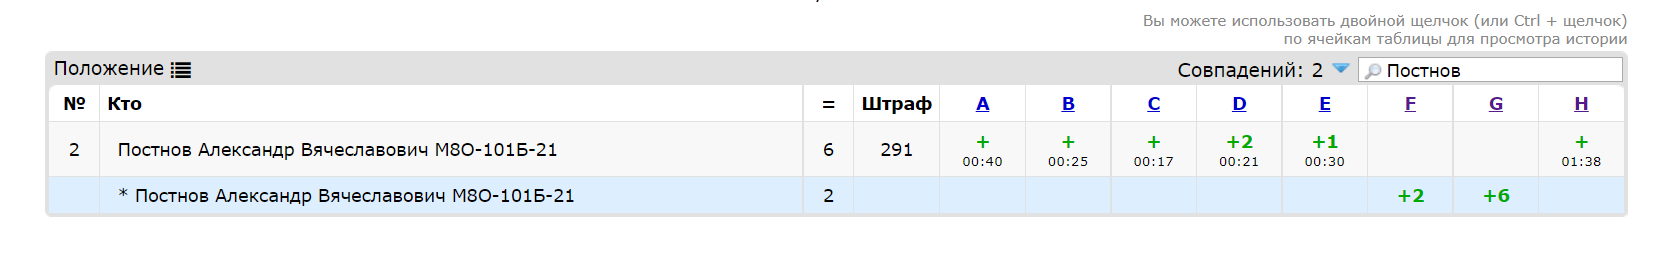
\includegraphics[width=\textwidth]{standings/14.png}\newline\noindent
\end{center}

\subsubsection*{Вывод}
Задача дорешена.

\vspace{20pt}

\pagebreak

\subsection*{СНМ, минимальное остовное дерево [13]}
\begin{center}
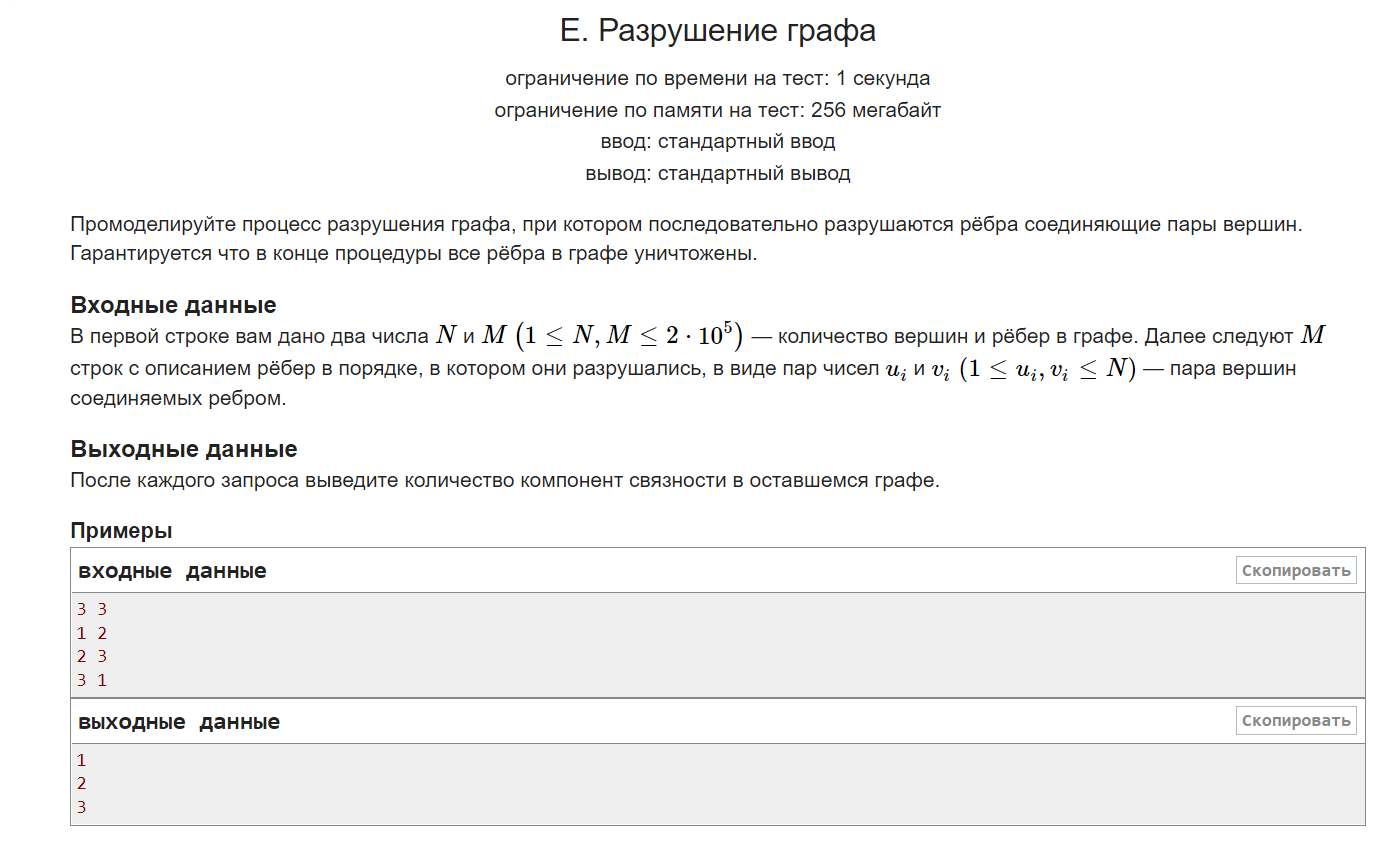
\includegraphics[width=\textwidth]{statements/15.png}
\end{center}
\subsubsection*{Идея решения}
Строим граф в обратном порядке, выписывая компонент связности графа, используя СНМ.
\subsubsection*{Исходный код}
\lstinputlisting{src/15.cpp}

\subsubsection*{Фрагмент турнирной таблицы контеста}
\begin{center}
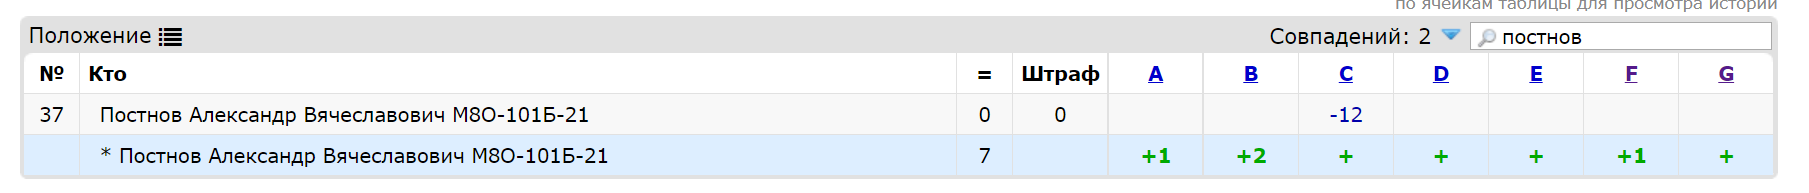
\includegraphics[width=\textwidth]{standings/15.png}\newline\noindent
\end{center}

\subsubsection*{Вывод}
Задача дорешена.

\vspace{20pt}

\pagebreak

\subsection*{Деревья, наименьший общий предок [14]}
\begin{center}
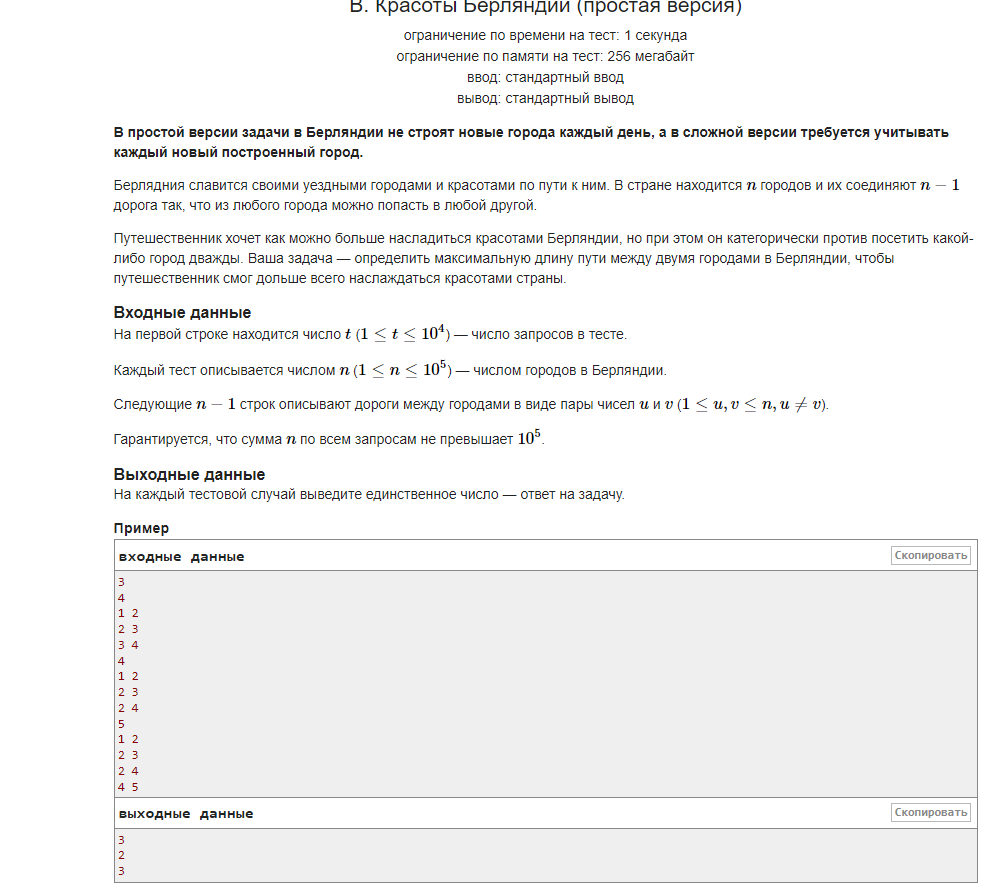
\includegraphics[width=\textwidth]{statements/16.png}
\end{center}
\subsubsection*{Идея решения}
Для того, чтобы определить максимальное расстояние между городами, использовать 2 раза алгоритм bfs. 1 раз применяем с любой вершины графа, а 2 раз с максимальным расстоянием от неё. В массиве dist после использования bfs будет находится ответ. 
Итоговая сложность: $O(n)$.
\subsubsection*{Исходный код}
\lstinputlisting{src/16.cpp}

\subsubsection*{Фрагмент турнирной таблицы контеста}
\begin{center}
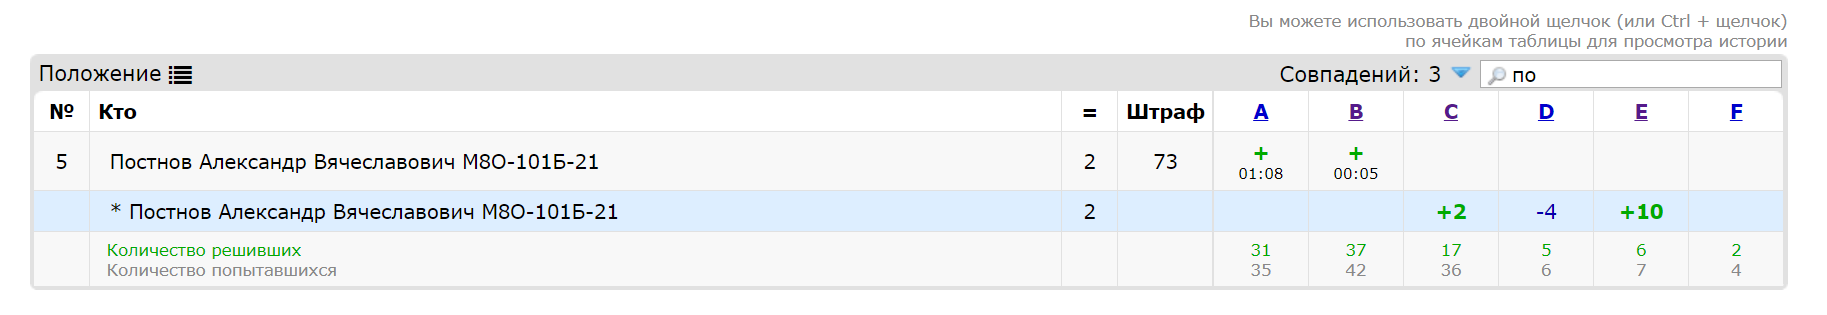
\includegraphics[width=\textwidth]{standings/16.png}\newline\noindent
\end{center}

\subsubsection*{Вывод}
Задача решена.

\vspace{20pt}

\pagebreak

\subsection*{Паросочетания в двудольном графе, потоки в транспортной сети [15]}
\begin{center}
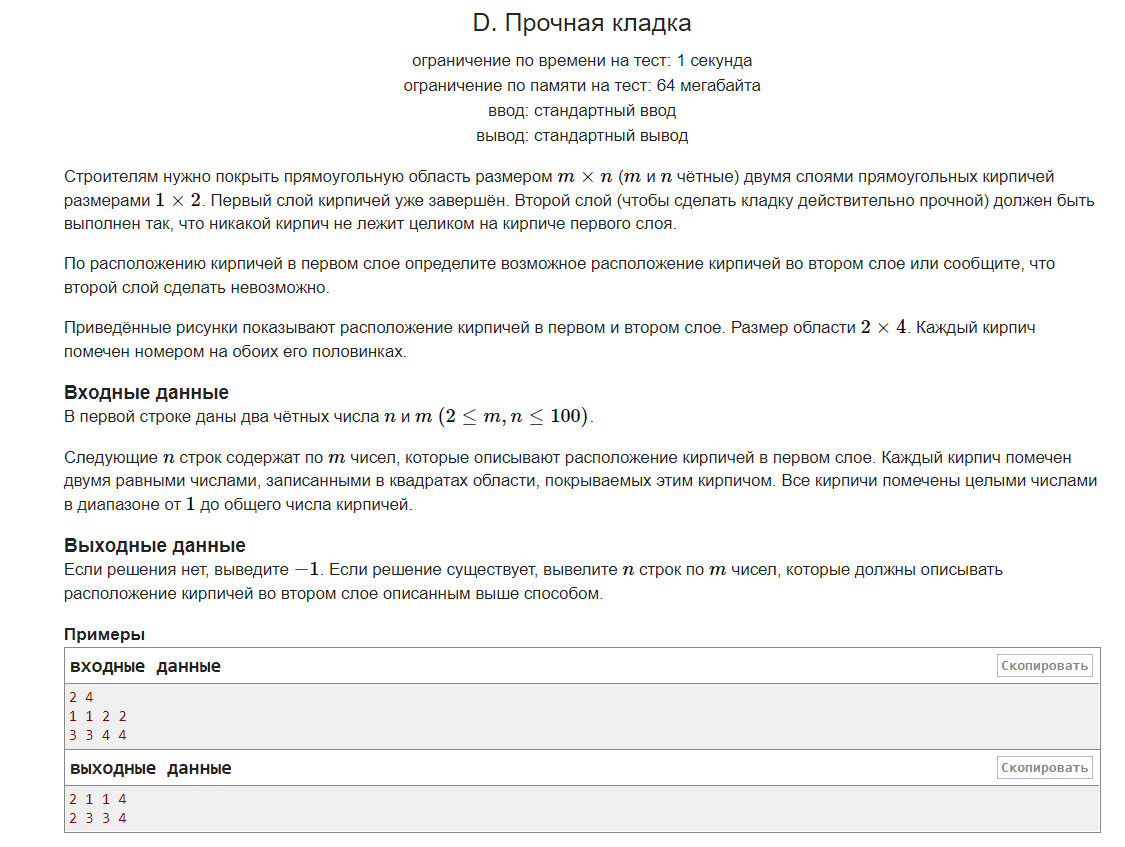
\includegraphics[width=\textwidth]{statements/17.png}
\end{center}
\subsubsection*{Идея решения}
Каждый кирпич будет вершиной графа, каждый кирпич будет связан с соседними кирпичами. Тогда необходимо просто максимальное паросочетание в этом графе и вывести в надобном порядке.
Итоговая сложность: $O(n*m)$
\subsubsection*{Исходный код}
\lstinputlisting{src/17.cpp}

\subsubsection*{Фрагмент турнирной таблицы контеста}
\begin{center}
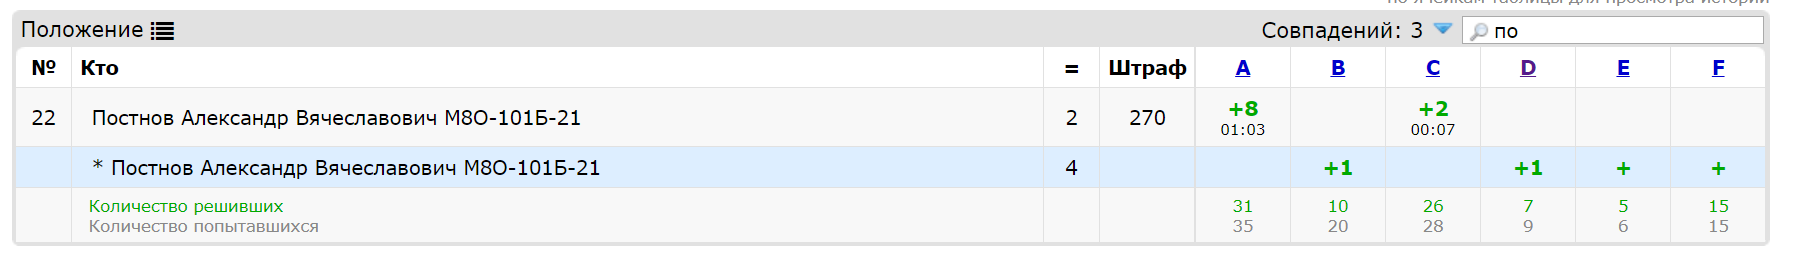
\includegraphics[width=\textwidth]{standings/17.png}\newline\noindent
\end{center}

\subsubsection*{Вывод}
Задача дорешена.

\vspace{20pt}

\pagebreak

\subsection*{Строки, Z-функция, хеши, префиксное дерево [16]}
\begin{center}
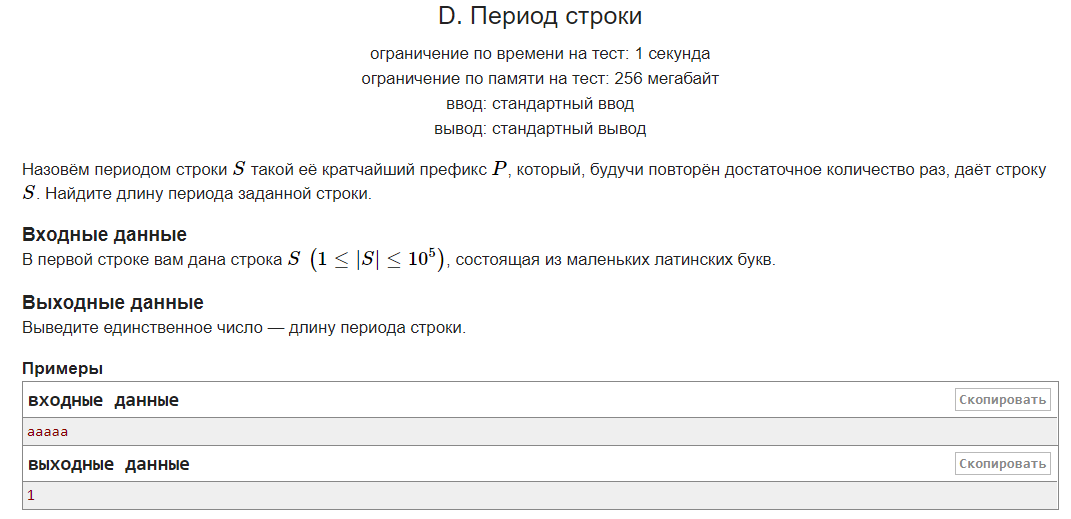
\includegraphics[width=\textwidth]{statements/18.png}
\end{center}
\subsubsection*{Идея решения}
В этой задаче необходимо использовать z-фунцию строки. Тогда, чтобы определить период, необходимо пройтись по строке, и если номер символа + значение z-функции == значению z-функции для 1 символа и период + период <= размеру строки, то ответ найден.
Итоговая сложность: $O(n)$
\subsubsection*{Исходный код}
\lstinputlisting{src/18.cpp}

\subsubsection*{Фрагмент турнирной таблицы контеста}
\begin{center}
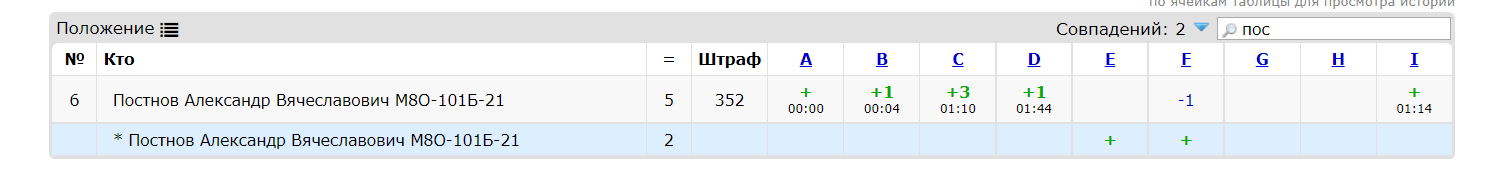
\includegraphics[width=\textwidth]{standings/18.png}\newline\noindent
\end{center}

\subsubsection*{Вывод}
Задача решена.

\vspace{20pt}

\pagebreak

\subsection*{ДП по подмножествам, ДП по профилю [17]}
\begin{center}
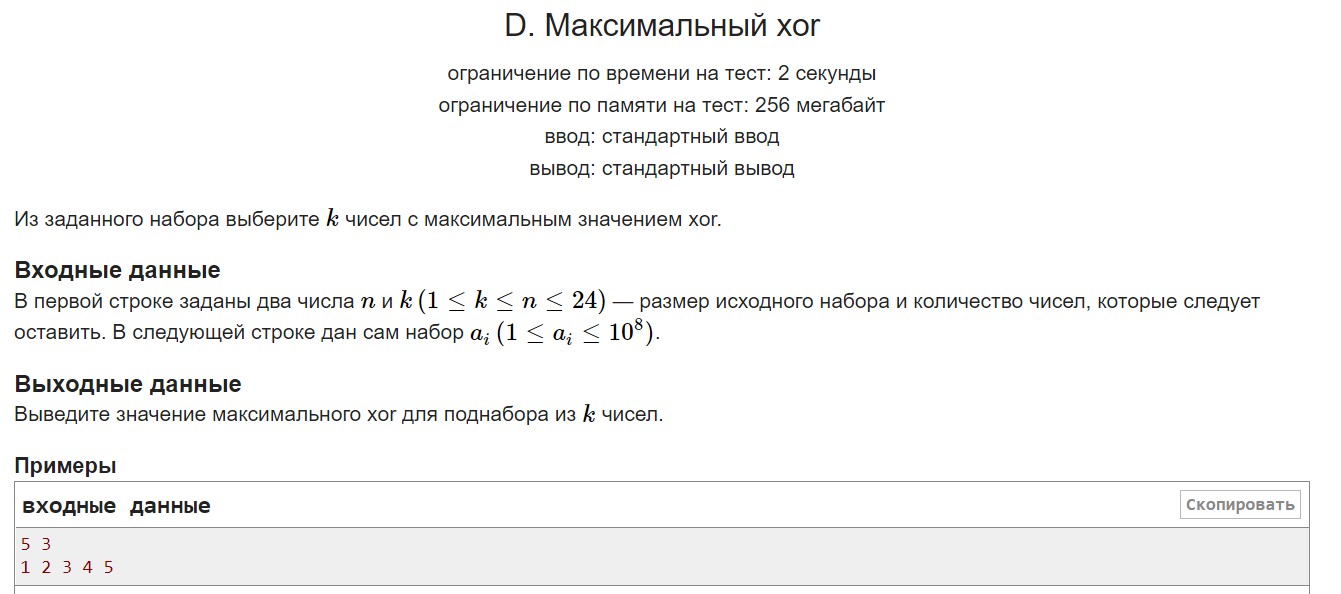
\includegraphics[width=\textwidth]{statements/19.png}
\end{center}
\subsubsection*{Идея решения}
В этой задаче нельзя использовать какой-либо алгоритм кроме полного перебора. Перебор будет производиться с помощью двоичной маски, где $0$ - не берем в набор, а $1$ - берем. Кол-во единиц должно быть равно $k$. 
Итоговая сложность: $O(n*2^n)$
\subsubsection*{Исходный код}
\lstinputlisting{src/19.cpp}

\subsubsection*{Фрагмент турнирной таблицы контеста}
\begin{center}
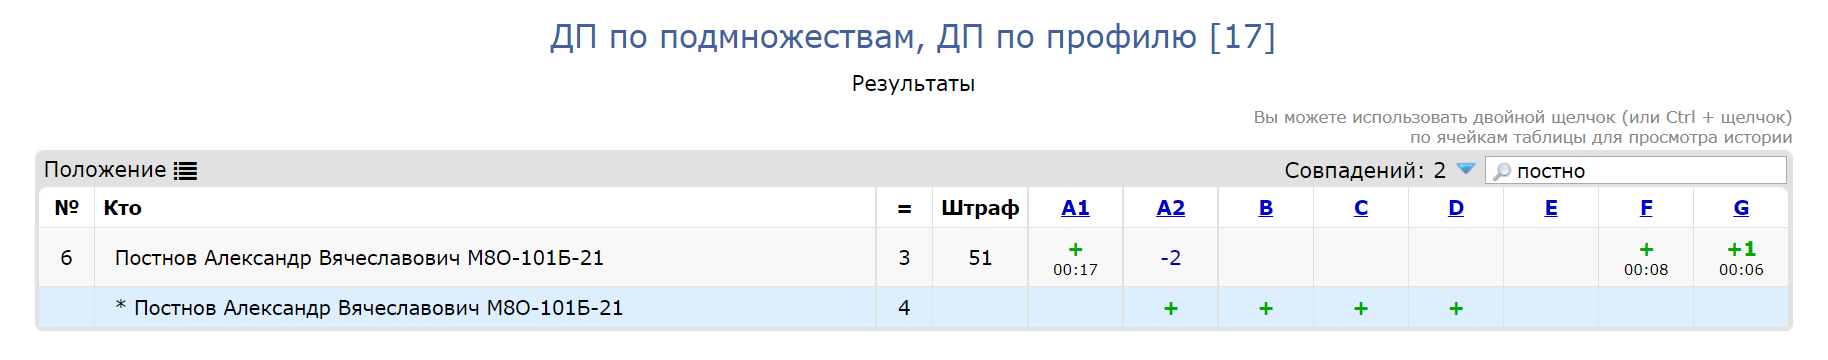
\includegraphics[width=\textwidth]{standings/19.png}\newline\noindent
\end{center}

\subsubsection*{Вывод}
Задача дорешена.

\vspace{20pt}

\pagebreak

\subsection*{Теория игр, функция Шпрага-Гранди [18]}
\begin{center}
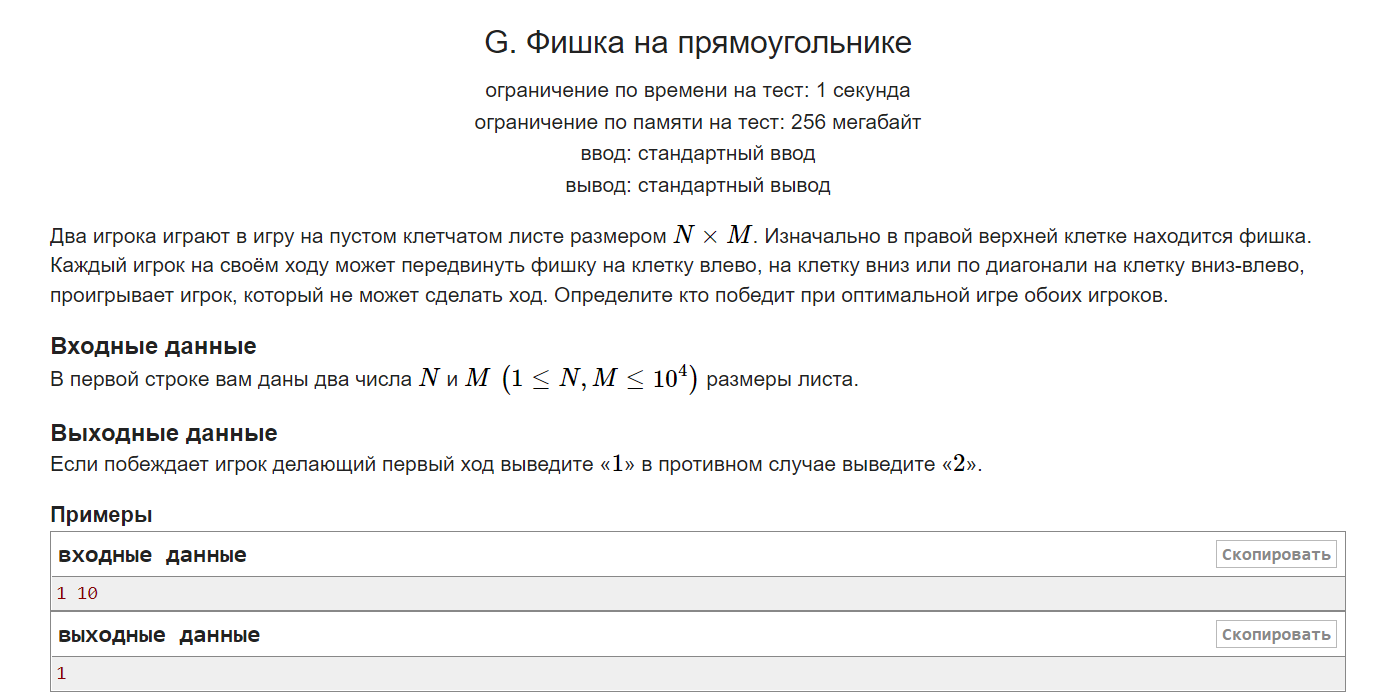
\includegraphics[width=\textwidth]{statements/20.png}
\end{center}
\subsubsection*{Идея решения}
После построения массива по функции Гранди можно заметить закономерность, если $n, m$ - нечетные, то побеждает 2 игрок, иначе - первый.
\subsubsection*{Исходный код}
\lstinputlisting{src/20.cpp}

\subsubsection*{Фрагмент турнирной таблицы контеста}
\begin{center}
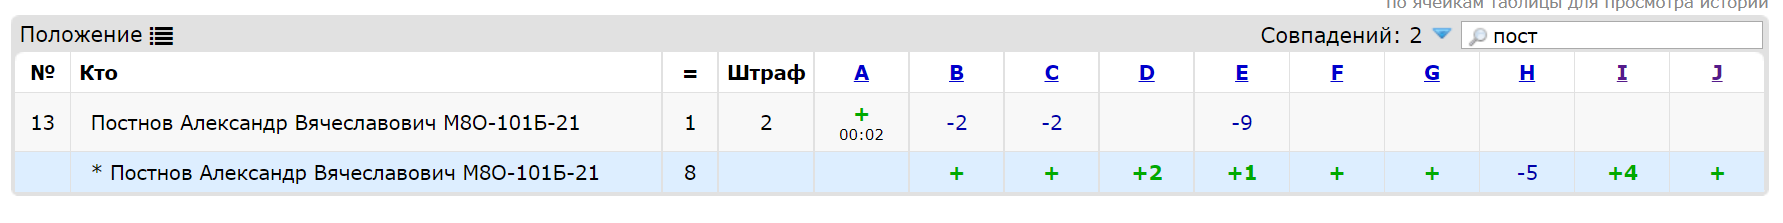
\includegraphics[width=\textwidth]{standings/20.png}\newline\noindent
\end{center}

\subsubsection*{Вывод}
Задача дорешена.

\vspace{20pt}

\pagebreak

\subsection*{Дерево отрезков [19]}
\begin{center}
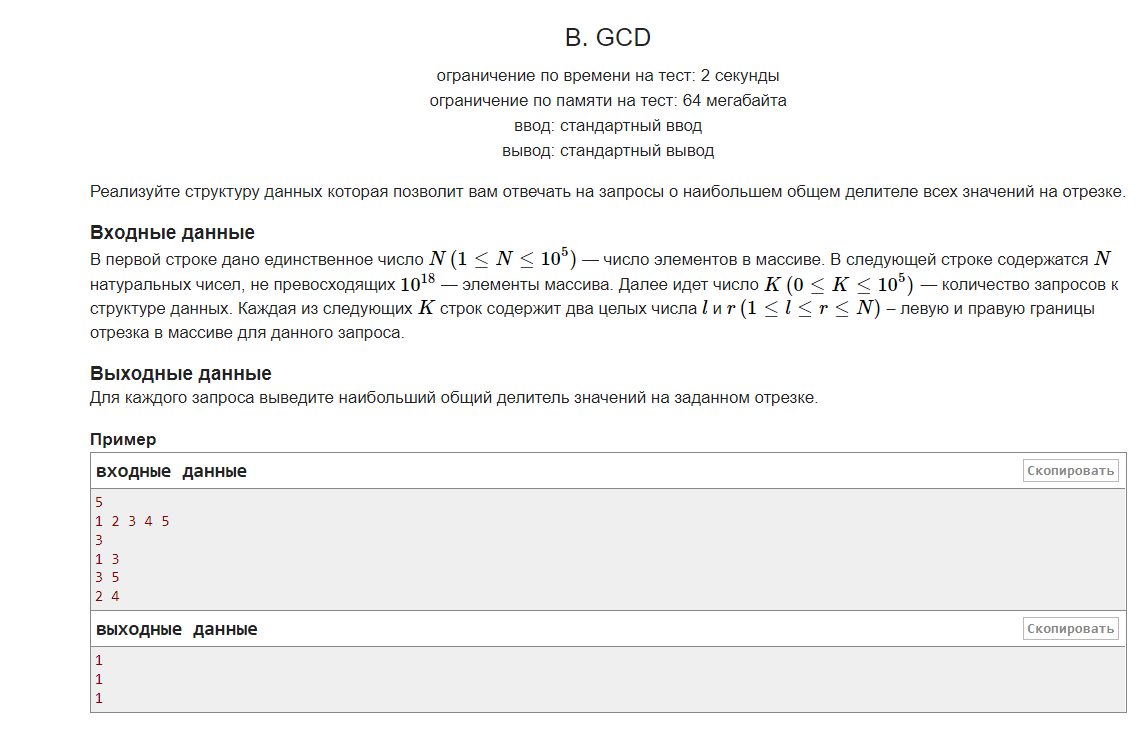
\includegraphics[width=\textwidth]{statements/21.png}
\end{center}
\subsubsection*{Идея решения}
Для эффективного решения буду использовать дерево отрезков. Поскольку операция gcd ассоциативна ДО можно использовать. Построение ДО - $O(n*log_{2} n)$, нахождение gcd на отрезке - $O(log_{2} n)$
\subsubsection*{Исходный код}
\lstinputlisting{src/21.cpp}

\subsubsection*{Фрагмент турнирной таблицы контеста}
\begin{center}
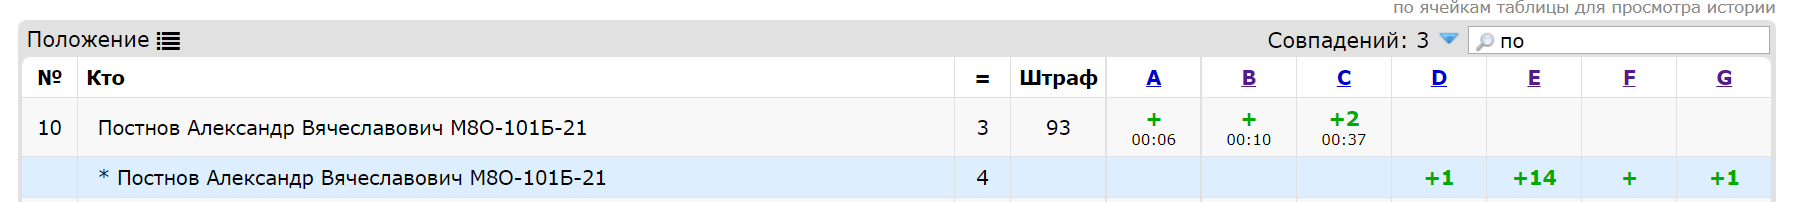
\includegraphics[width=\textwidth]{standings/21.png}\newline\noindent
\end{center}

\subsubsection*{Вывод}
Задача решена.

\vspace{20pt}

\pagebreak

\subsection*{Декартово дерево [21]}
\begin{center}
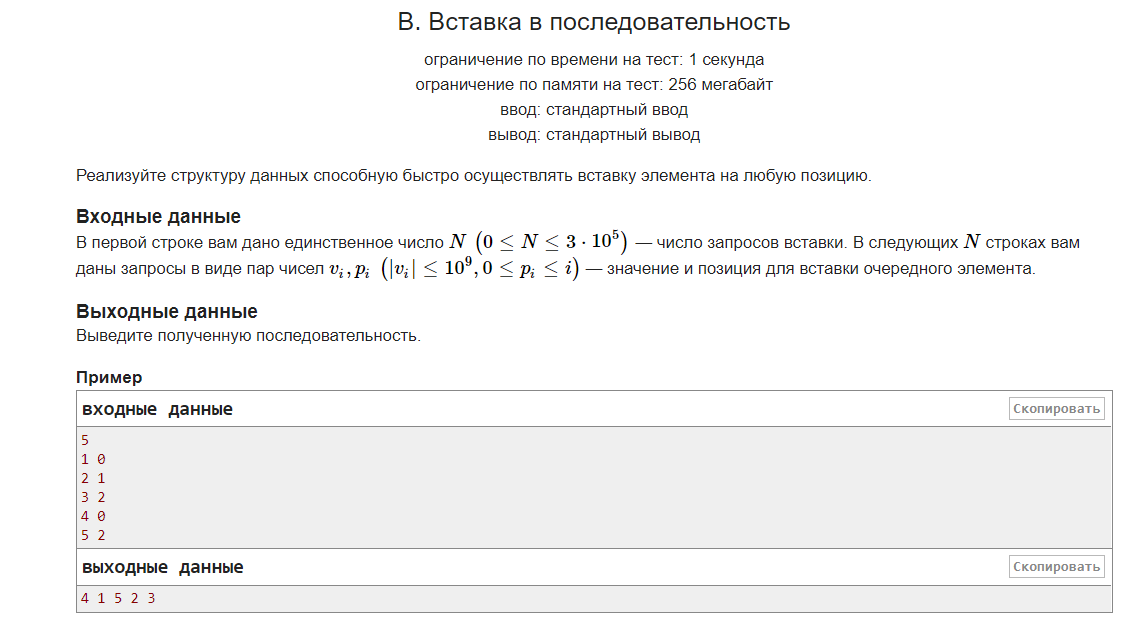
\includegraphics[width=\textwidth]{statements/22.png}
\end{center}
\subsubsection*{Идея решения}
В этой задаче я буду использовать такую структуру данных, как Декартово дерево. Вставка элементов по ключу(в данном случае по позиции) имеет сложность $O(log_{2} n)$. Вставка должна использоваться $n$ раз. Итоговая сложность: $O(n*log_{2} n)$
\subsubsection*{Исходный код}
\lstinputlisting{src/22.cpp}

\subsubsection*{Фрагмент турнирной таблицы контеста}
\begin{center}
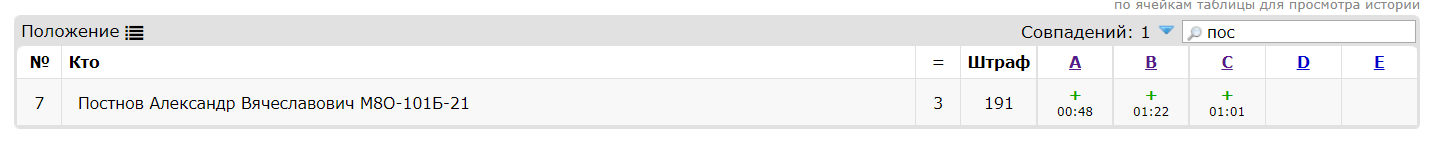
\includegraphics[width=\textwidth]{standings/22.png}\newline\noindent
\end{center}

\subsubsection*{Вывод}
Задача решена.

\vspace{20pt}

\pagebreak


\subsection*{Весенняя олимпиада первого курса}
\begin{center}
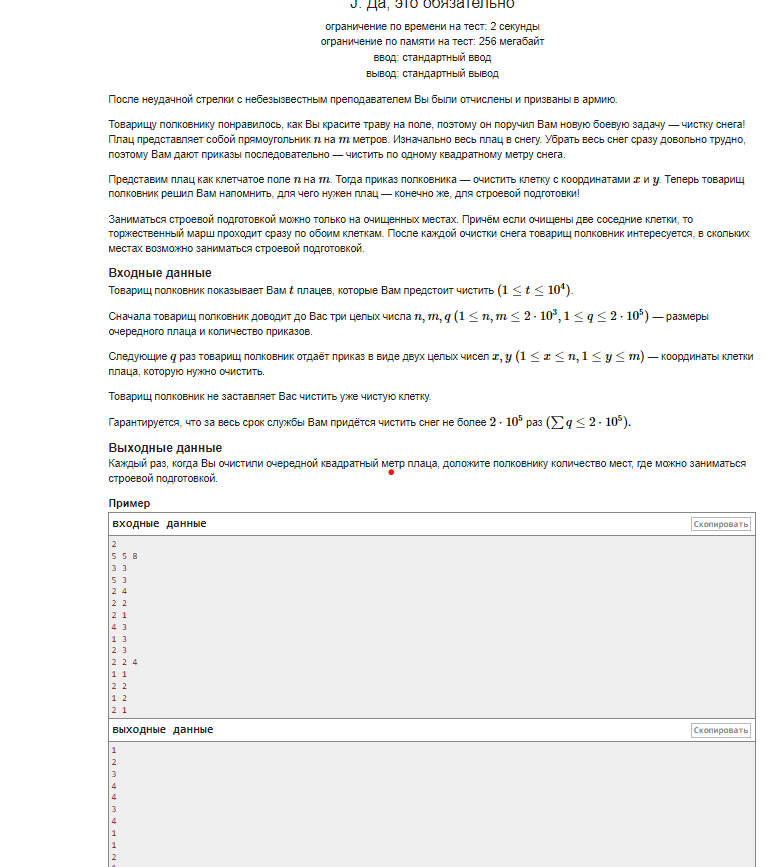
\includegraphics[width=\textwidth]{statements/23.png}
\end{center}
\subsubsection*{Идея решения}
Буду использовать СНМ, представлю клетки как вершины графа. Как только очищаю клетку(к итоговому ответу ++), смотрю влево, вправо, вверх, вниз, если клетка тоже очищена и лидер с текущей клеткой разный, то объединяю эти множества и отнимаю от ответа 1.
Итоговая сложность: $O(t*(n*m + q*\alpha(n*m))$
\subsubsection*{Исходный код}
\lstinputlisting{src/23.cpp}

\subsubsection*{Фрагмент турнирной таблицы контеста}
\begin{center}
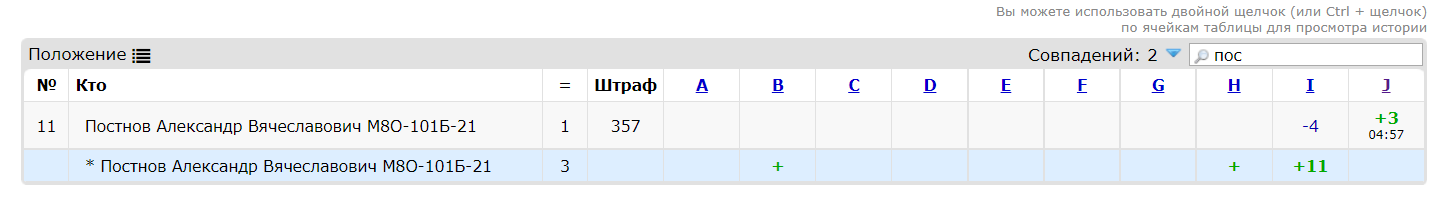
\includegraphics[width=\textwidth]{standings/23.png}\newline\noindent
\end{center}

\subsubsection*{Вывод}
В ходе практики изучил классические алгоритмы по обработке строк, графов. Изучил идею динамического программирования, улучшил знания по теории чисел, изучил новые для себя типы данных: дерево отрезков, декартово дерево, префиксное дерево. Подтянул навыки аналитической геометрии. А также улучшил навыки работы с LaTeX, написав отчет на нем. Думаю, что полученные знания мне пригодятся в будущем!

\vspace{20pt}

\pagebreak